\documentclass[twoside]{book}

% Packages required by doxygen
\usepackage{fixltx2e}
\usepackage{calc}
\usepackage{doxygen}
\usepackage[export]{adjustbox} % also loads graphicx
\usepackage{graphicx}
\usepackage[utf8]{inputenc}
\usepackage{makeidx}
\usepackage{multicol}
\usepackage{multirow}
\PassOptionsToPackage{warn}{textcomp}
\usepackage{textcomp}
\usepackage[nointegrals]{wasysym}
\usepackage[table]{xcolor}

% Font selection
\usepackage[T1]{fontenc}
\usepackage[scaled=.90]{helvet}
\usepackage{courier}
\usepackage{amssymb}
\usepackage{sectsty}
\renewcommand{\familydefault}{\sfdefault}
\allsectionsfont{%
  \fontseries{bc}\selectfont%
  \color{darkgray}%
}
\renewcommand{\DoxyLabelFont}{%
  \fontseries{bc}\selectfont%
  \color{darkgray}%
}
\newcommand{\+}{\discretionary{\mbox{\scriptsize$\hookleftarrow$}}{}{}}

% Page & text layout
\usepackage{geometry}
\geometry{%
  a4paper,%
  top=2.5cm,%
  bottom=2.5cm,%
  left=2.5cm,%
  right=2.5cm%
}
\tolerance=750
\hfuzz=15pt
\hbadness=750
\setlength{\emergencystretch}{15pt}
\setlength{\parindent}{0cm}
\setlength{\parskip}{3ex plus 2ex minus 2ex}
\makeatletter
\renewcommand{\paragraph}{%
  \@startsection{paragraph}{4}{0ex}{-1.0ex}{1.0ex}{%
    \normalfont\normalsize\bfseries\SS@parafont%
  }%
}
\renewcommand{\subparagraph}{%
  \@startsection{subparagraph}{5}{0ex}{-1.0ex}{1.0ex}{%
    \normalfont\normalsize\bfseries\SS@subparafont%
  }%
}
\makeatother

% Headers & footers
\usepackage{fancyhdr}
\pagestyle{fancyplain}
\fancyhead[LE]{\fancyplain{}{\bfseries\thepage}}
\fancyhead[CE]{\fancyplain{}{}}
\fancyhead[RE]{\fancyplain{}{\bfseries\leftmark}}
\fancyhead[LO]{\fancyplain{}{\bfseries\rightmark}}
\fancyhead[CO]{\fancyplain{}{}}
\fancyhead[RO]{\fancyplain{}{\bfseries\thepage}}
\fancyfoot[LE]{\fancyplain{}{}}
\fancyfoot[CE]{\fancyplain{}{}}
\fancyfoot[RE]{\fancyplain{}{\bfseries\scriptsize Generated by Doxygen }}
\fancyfoot[LO]{\fancyplain{}{\bfseries\scriptsize Generated by Doxygen }}
\fancyfoot[CO]{\fancyplain{}{}}
\fancyfoot[RO]{\fancyplain{}{}}
\renewcommand{\footrulewidth}{0.4pt}
\renewcommand{\chaptermark}[1]{%
  \markboth{#1}{}%
}
\renewcommand{\sectionmark}[1]{%
  \markright{\thesection\ #1}%
}

% Indices & bibliography
\usepackage{natbib}
\usepackage[titles]{tocloft}
\setcounter{tocdepth}{3}
\setcounter{secnumdepth}{5}
\makeindex

% Hyperlinks (required, but should be loaded last)
\usepackage{ifpdf}
\ifpdf
  \usepackage[pdftex,pagebackref=true]{hyperref}
\else
  \usepackage[ps2pdf,pagebackref=true]{hyperref}
\fi
\hypersetup{%
  colorlinks=true,%
  linkcolor=blue,%
  citecolor=blue,%
  unicode%
}

% Custom commands
\newcommand{\clearemptydoublepage}{%
  \newpage{\pagestyle{empty}\cleardoublepage}%
}

\usepackage{caption}
\captionsetup{labelsep=space,justification=centering,font={bf},singlelinecheck=off,skip=4pt,position=top}

%===== C O N T E N T S =====

\begin{document}

% Titlepage & ToC
\hypersetup{pageanchor=false,
             bookmarksnumbered=true,
             pdfencoding=unicode
            }
\pagenumbering{alph}
\begin{titlepage}
\vspace*{7cm}
\begin{center}%
{\Large Implémentation d\textquotesingle{}un container multimap en C++ }\\
\vspace*{1cm}
{\large Generated by Doxygen 1.8.13}\\
\end{center}
\end{titlepage}
\clearemptydoublepage
\pagenumbering{roman}
\tableofcontents
\clearemptydoublepage
\pagenumbering{arabic}
\hypersetup{pageanchor=true}

%--- Begin generated contents ---
\chapter{Namespace Index}
\section{Namespace List}
Here is a list of all documented namespaces with brief descriptions\+:\begin{DoxyCompactList}
\item\contentsline{section}{\hyperlink{namespaceimpl}{impl} }{\pageref{namespaceimpl}}{}
\item\contentsline{section}{\hyperlink{namespacepair__operators}{pair\+\_\+operators} \\*Namespace qui défini des fonctions sur le type std\+::pair }{\pageref{namespacepair__operators}}{}
\item\contentsline{section}{\hyperlink{namespacetraits}{traits} }{\pageref{namespacetraits}}{}
\end{DoxyCompactList}

\chapter{Hierarchical Index}
\section{Class Hierarchy}
This inheritance list is sorted roughly, but not completely, alphabetically\+:\begin{DoxyCompactList}
\item \contentsline{section}{add\+\_\+const\+\_\+if$<$ Is\+Const, T $>$}{\pageref{structadd__const__if}}{}
\item \contentsline{section}{add\+\_\+const\+\_\+if$<$ true, T $>$}{\pageref{structadd__const__if_3_01true_00_01T_01_4}}{}
\item \contentsline{section}{B\+S\+Tree$<$ T, N $>$}{\pageref{classBSTree}}{}
\item \contentsline{section}{B\+S\+Tree$<$ List$<$ value\+\_\+type $>$ $>$}{\pageref{classBSTree}}{}
\item \contentsline{section}{B\+S\+Tree\+Node$<$ T, Node $>$}{\pageref{classBSTreeNode}}{}
\item \contentsline{section}{B\+S\+Tree\+Node$<$ T, Binary\+Node$<$ T $>$ $>$}{\pageref{classBSTreeNode}}{}
\begin{DoxyCompactList}
\item \contentsline{section}{Binary\+Node$<$ T $>$}{\pageref{classBinaryNode}}{}
\end{DoxyCompactList}
\item \contentsline{section}{Counter}{\pageref{classCounter}}{}
\item \contentsline{section}{Custom\+Comparator$<$ Key $>$}{\pageref{structCustomComparator}}{}
\item \contentsline{section}{Custom\+Type}{\pageref{structCustomType}}{}
\item \contentsline{section}{traits\+:\+:is\+\_\+multimap$<$ T, V $>$}{\pageref{structtraits_1_1is__multimap}}{}
\item \contentsline{section}{traits\+:\+:is\+\_\+multimap$<$ Multimap$<$ T, U, V $>$, W $>$}{\pageref{structtraits_1_1is__multimap_3_01Multimap_3_01T_00_01U_00_01V_01_4_00_01W_01_4}}{}
\item \contentsline{section}{traits\+:\+:is\+\_\+multimap$<$ std\+:\+:multimap$<$ T, U, V $>$, W $>$}{\pageref{structtraits_1_1is__multimap_3_01std_1_1multimap_3_01T_00_01U_00_01V_01_4_00_01W_01_4}}{}
\item \contentsline{section}{List$<$ T $>$}{\pageref{classList}}{}
\item \contentsline{section}{List\+Node$<$ T $>$}{\pageref{classListNode}}{}
\item logic\+\_\+error\begin{DoxyCompactList}
\item \contentsline{section}{Assertion\+Error}{\pageref{classAssertionError}}{}
\end{DoxyCompactList}
\item \contentsline{section}{Map$<$ Key, T $>$}{\pageref{classMap}}{}
\item \contentsline{section}{Map\+Iterator$<$ Key, T $>$}{\pageref{classMapIterator}}{}
\item \contentsline{section}{Multimap$<$ Key, T, Compare $>$}{\pageref{classMultimap}}{}
\item \contentsline{section}{Multimap\+Iterator$<$ Key, Value, Compare, Is\+Const $>$}{\pageref{classMultimapIterator}}{}
\item \contentsline{section}{rb\+\_\+iter}{\pageref{structrb__iter}}{}
\item \contentsline{section}{rb\+\_\+node}{\pageref{structrb__node}}{}
\item \contentsline{section}{rb\+\_\+tree}{\pageref{structrb__tree}}{}
\item \contentsline{section}{impl\+:\+:Test\+Count$<$ I, bool $>$}{\pageref{structimpl_1_1TestCount}}{}
\item \contentsline{section}{impl\+:\+:Test\+Count$<$ I, false $>$}{\pageref{structimpl_1_1TestCount_3_01I_00_01false_01_4}}{}
\item \contentsline{section}{impl\+:\+:Test\+Count$<$ I, true $>$}{\pageref{structimpl_1_1TestCount_3_01I_00_01true_01_4}}{}
\item \contentsline{section}{Test\+Suite$<$ N $>$}{\pageref{structTestSuite}}{}
\item \contentsline{section}{Test\+Suite$<$ 0 $>$}{\pageref{structTestSuite_3_010_01_4}}{}
\item \contentsline{section}{Test\+Suite$<$ 1 $>$}{\pageref{structTestSuite_3_011_01_4}}{}
\item \contentsline{section}{Multimap$<$ Key, T, Compare $>$\+:\+:value\+\_\+compare}{\pageref{classMultimap_1_1value__compare}}{}
\end{DoxyCompactList}

\chapter{Class Index}
\section{Class List}
Here are the classes, structs, unions and interfaces with brief descriptions\+:\begin{DoxyCompactList}
\item\contentsline{section}{\hyperlink{structadd__const__if}{add\+\_\+const\+\_\+if$<$ Is\+Const, T $>$} }{\pageref{structadd__const__if}}{}
\item\contentsline{section}{\hyperlink{structadd__const__if_3_01true_00_01T_01_4}{add\+\_\+const\+\_\+if$<$ true, T $>$} }{\pageref{structadd__const__if_3_01true_00_01T_01_4}}{}
\item\contentsline{section}{\hyperlink{classAssertionError}{Assertion\+Error} \\*Exception lancéé en cas d\textquotesingle{}assertion non vérifiée }{\pageref{classAssertionError}}{}
\item\contentsline{section}{\hyperlink{classBinaryNode}{Binary\+Node$<$ T $>$} }{\pageref{classBinaryNode}}{}
\item\contentsline{section}{\hyperlink{classBSTree}{B\+S\+Tree$<$ T, N $>$} \\*Arbre contenant des noeuds génériques }{\pageref{classBSTree}}{}
\item\contentsline{section}{\hyperlink{classBSTreeNode}{B\+S\+Tree\+Node$<$ T, Node $>$} }{\pageref{classBSTreeNode}}{}
\item\contentsline{section}{\hyperlink{classCounter}{Counter} }{\pageref{classCounter}}{}
\item\contentsline{section}{\hyperlink{structCustomComparator}{Custom\+Comparator$<$ Key $>$} }{\pageref{structCustomComparator}}{}
\item\contentsline{section}{\hyperlink{structCustomType}{Custom\+Type} }{\pageref{structCustomType}}{}
\item\contentsline{section}{\hyperlink{structtraits_1_1is__multimap}{traits\+::is\+\_\+multimap$<$ T, V $>$} }{\pageref{structtraits_1_1is__multimap}}{}
\item\contentsline{section}{\hyperlink{structtraits_1_1is__multimap_3_01Multimap_3_01T_00_01U_00_01V_01_4_00_01W_01_4}{traits\+::is\+\_\+multimap$<$ Multimap$<$ T, U, V $>$, W $>$} }{\pageref{structtraits_1_1is__multimap_3_01Multimap_3_01T_00_01U_00_01V_01_4_00_01W_01_4}}{}
\item\contentsline{section}{\hyperlink{structtraits_1_1is__multimap_3_01std_1_1multimap_3_01T_00_01U_00_01V_01_4_00_01W_01_4}{traits\+::is\+\_\+multimap$<$ std\+::multimap$<$ T, U, V $>$, W $>$} }{\pageref{structtraits_1_1is__multimap_3_01std_1_1multimap_3_01T_00_01U_00_01V_01_4_00_01W_01_4}}{}
\item\contentsline{section}{\hyperlink{classList}{List$<$ T $>$} }{\pageref{classList}}{}
\item\contentsline{section}{\hyperlink{classListNode}{List\+Node$<$ T $>$} }{\pageref{classListNode}}{}
\item\contentsline{section}{\hyperlink{classMap}{Map$<$ Key, T $>$} }{\pageref{classMap}}{}
\item\contentsline{section}{\hyperlink{classMapIterator}{Map\+Iterator$<$ Key, T $>$} }{\pageref{classMapIterator}}{}
\item\contentsline{section}{\hyperlink{classMultimap}{Multimap$<$ Key, T, Compare $>$} }{\pageref{classMultimap}}{}
\item\contentsline{section}{\hyperlink{classMultimapIterator}{Multimap\+Iterator$<$ Key, Value, Compare, Is\+Const $>$} \\*Itérateur }{\pageref{classMultimapIterator}}{}
\item\contentsline{section}{\hyperlink{structrb__iter}{rb\+\_\+iter} }{\pageref{structrb__iter}}{}
\item\contentsline{section}{\hyperlink{structrb__node}{rb\+\_\+node} }{\pageref{structrb__node}}{}
\item\contentsline{section}{\hyperlink{structrb__tree}{rb\+\_\+tree} }{\pageref{structrb__tree}}{}
\item\contentsline{section}{\hyperlink{structimpl_1_1TestCount}{impl\+::\+Test\+Count$<$ I, bool $>$} }{\pageref{structimpl_1_1TestCount}}{}
\item\contentsline{section}{\hyperlink{structimpl_1_1TestCount_3_01I_00_01false_01_4}{impl\+::\+Test\+Count$<$ I, false $>$} }{\pageref{structimpl_1_1TestCount_3_01I_00_01false_01_4}}{}
\item\contentsline{section}{\hyperlink{structimpl_1_1TestCount_3_01I_00_01true_01_4}{impl\+::\+Test\+Count$<$ I, true $>$} }{\pageref{structimpl_1_1TestCount_3_01I_00_01true_01_4}}{}
\item\contentsline{section}{\hyperlink{structTestSuite}{Test\+Suite$<$ N $>$} }{\pageref{structTestSuite}}{}
\item\contentsline{section}{\hyperlink{structTestSuite_3_010_01_4}{Test\+Suite$<$ 0 $>$} }{\pageref{structTestSuite_3_010_01_4}}{}
\item\contentsline{section}{\hyperlink{structTestSuite_3_011_01_4}{Test\+Suite$<$ 1 $>$} }{\pageref{structTestSuite_3_011_01_4}}{}
\item\contentsline{section}{\hyperlink{classMultimap_1_1value__compare}{Multimap$<$ Key, T, Compare $>$\+::value\+\_\+compare} \\*Classe qui compare les paires }{\pageref{classMultimap_1_1value__compare}}{}
\end{DoxyCompactList}

\chapter{Namespace Documentation}
\hypertarget{namespaceimpl}{}\section{impl Namespace Reference}
\label{namespaceimpl}\index{impl@{impl}}
\subsection*{Classes}
\begin{DoxyCompactItemize}
\item 
struct \hyperlink{structimpl_1_1TestCount}{Test\+Count}
\item 
struct \hyperlink{structimpl_1_1TestCount_3_01I_00_01false_01_4}{Test\+Count$<$ I, false $>$}
\item 
struct \hyperlink{structimpl_1_1TestCount_3_01I_00_01true_01_4}{Test\+Count$<$ I, true $>$}
\end{DoxyCompactItemize}
\subsection*{Functions}
\begin{DoxyCompactItemize}
\item 
\mbox{\Hypertarget{namespaceimpl_a7906d56174d1e06fb4a702e0b10905d3}\label{namespaceimpl_a7906d56174d1e06fb4a702e0b10905d3}} 
{\footnotesize template$<$typename T $>$ }\\constexpr bool {\bfseries test\+Exists} (decltype(T\+::empty\+Test, int()))
\item 
\mbox{\Hypertarget{namespaceimpl_a7bdf37b41f6d1d93a26a8077934a4ccd}\label{namespaceimpl_a7bdf37b41f6d1d93a26a8077934a4ccd}} 
{\footnotesize template$<$typename T $>$ }\\constexpr bool {\bfseries test\+Exists} (long)
\item 
\mbox{\Hypertarget{namespaceimpl_afbea0170e33aad3040d0a3e7fbdb3c3d}\label{namespaceimpl_afbea0170e33aad3040d0a3e7fbdb3c3d}} 
{\footnotesize template$<$typename T $>$ }\\constexpr bool {\bfseries test\+Exists} ()
\end{DoxyCompactItemize}


\subsection{Detailed Description}
Implémentation du compteur de test. 
\hypertarget{namespacepair__operators}{}\section{pair\+\_\+operators Namespace Reference}
\label{namespacepair__operators}\index{pair\+\_\+operators@{pair\+\_\+operators}}


Namespace qui défini des fonctions sur le type std\+::pair.  


\subsection*{Functions}
\begin{DoxyCompactItemize}
\item 
\mbox{\Hypertarget{namespacepair__operators_a115d8bbb7c2e8a55ff76ead25ea47da5}\label{namespacepair__operators_a115d8bbb7c2e8a55ff76ead25ea47da5}} 
{\footnotesize template$<$typename U , typename V $>$ }\\std\+::ostream \& \hyperlink{namespacepair__operators_a115d8bbb7c2e8a55ff76ead25ea47da5}{operator$<$$<$} (std\+::ostream \&lhs, const std\+::pair$<$ U, V $>$ \&pair)
\begin{DoxyCompactList}\small\item\em Affichage d\textquotesingle{}une paire sous forme \{\char`\"{}first value\char`\"{}, \char`\"{}second value\char`\"{}\}. \end{DoxyCompactList}\end{DoxyCompactItemize}


\subsection{Detailed Description}
Namespace qui défini des fonctions sur le type std\+::pair. 
\hypertarget{namespacetraits}{}\section{traits Namespace Reference}
\label{namespacetraits}\index{traits@{traits}}
\subsection*{Classes}
\begin{DoxyCompactItemize}
\item 
struct \hyperlink{structtraits_1_1is__multimap}{is\+\_\+multimap}
\item 
struct \hyperlink{structtraits_1_1is__multimap_3_01Multimap_3_01T_00_01U_00_01V_01_4_00_01W_01_4}{is\+\_\+multimap$<$ Multimap$<$ T, U, V $>$, W $>$}
\item 
struct \hyperlink{structtraits_1_1is__multimap_3_01std_1_1multimap_3_01T_00_01U_00_01V_01_4_00_01W_01_4}{is\+\_\+multimap$<$ std\+::multimap$<$ T, U, V $>$, W $>$}
\end{DoxyCompactItemize}
\subsection*{Typedefs}
\begin{DoxyCompactItemize}
\item 
\mbox{\Hypertarget{namespacetraits_a01e5b63ca6c09e48cdbdf814cbe498cc}\label{namespacetraits_a01e5b63ca6c09e48cdbdf814cbe498cc}} 
{\footnotesize template$<$typename T , typename V  = T$>$ }\\using {\bfseries is\+\_\+multimap\+\_\+t} = typename \hyperlink{structtraits_1_1is__multimap}{is\+\_\+multimap}$<$ T, V $>$\+::type
\end{DoxyCompactItemize}


\subsection{Detailed Description}
Traits de type 
\chapter{Class Documentation}
\hypertarget{structadd__const__if}{}\section{add\+\_\+const\+\_\+if$<$ Is\+Const, T $>$ Struct Template Reference}
\label{structadd__const__if}\index{add\+\_\+const\+\_\+if$<$ Is\+Const, T $>$@{add\+\_\+const\+\_\+if$<$ Is\+Const, T $>$}}
\subsection*{Public Types}
\begin{DoxyCompactItemize}
\item 
\mbox{\Hypertarget{structadd__const__if_a3e6643d31fba37bdb1d3ebeacb121723}\label{structadd__const__if_a3e6643d31fba37bdb1d3ebeacb121723}} 
typedef T {\bfseries type}
\end{DoxyCompactItemize}


The documentation for this struct was generated from the following file\+:\begin{DoxyCompactItemize}
\item 
src/multimap/Multimap\+Iterator.\+h\end{DoxyCompactItemize}

\hypertarget{structadd__const__if_3_01true_00_01T_01_4}{}\section{add\+\_\+const\+\_\+if$<$ true, T $>$ Struct Template Reference}
\label{structadd__const__if_3_01true_00_01T_01_4}\index{add\+\_\+const\+\_\+if$<$ true, T $>$@{add\+\_\+const\+\_\+if$<$ true, T $>$}}
\subsection*{Public Types}
\begin{DoxyCompactItemize}
\item 
\mbox{\Hypertarget{structadd__const__if_3_01true_00_01T_01_4_ac820eb899a0feed4f9605c6e80f8f857}\label{structadd__const__if_3_01true_00_01T_01_4_ac820eb899a0feed4f9605c6e80f8f857}} 
typedef const T {\bfseries type}
\end{DoxyCompactItemize}


The documentation for this struct was generated from the following file\+:\begin{DoxyCompactItemize}
\item 
src/multimap/Multimap\+Iterator.\+h\end{DoxyCompactItemize}

\hypertarget{classAssertionError}{}\section{Assertion\+Error Class Reference}
\label{classAssertionError}\index{Assertion\+Error@{Assertion\+Error}}


Exception lancéé en cas d\textquotesingle{}assertion non vérifiée.  




{\ttfamily \#include $<$Defines.\+h$>$}



Inheritance diagram for Assertion\+Error\+:\nopagebreak
\begin{figure}[H]
\begin{center}
\leavevmode
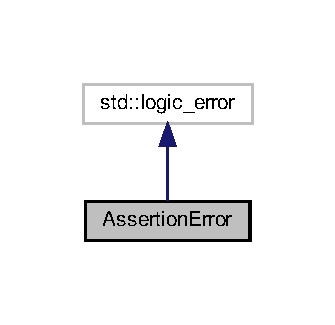
\includegraphics[width=161pt]{classAssertionError__inherit__graph}
\end{center}
\end{figure}


Collaboration diagram for Assertion\+Error\+:\nopagebreak
\begin{figure}[H]
\begin{center}
\leavevmode
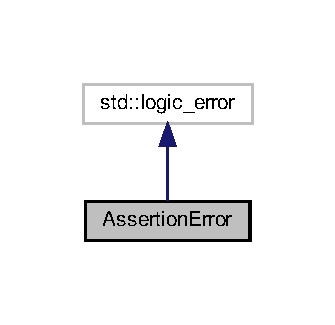
\includegraphics[width=161pt]{classAssertionError__coll__graph}
\end{center}
\end{figure}


\subsection{Detailed Description}
Exception lancéé en cas d\textquotesingle{}assertion non vérifiée. 

The documentation for this class was generated from the following file\+:\begin{DoxyCompactItemize}
\item 
src/Defines.\+h\end{DoxyCompactItemize}

\hypertarget{classBinaryNode}{}\section{Binary\+Node$<$ T $>$ Class Template Reference}
\label{classBinaryNode}\index{Binary\+Node$<$ T $>$@{Binary\+Node$<$ T $>$}}


{\ttfamily \#include $<$B\+S\+Tree.\+h$>$}



Inheritance diagram for Binary\+Node$<$ T $>$\+:\nopagebreak
\begin{figure}[H]
\begin{center}
\leavevmode
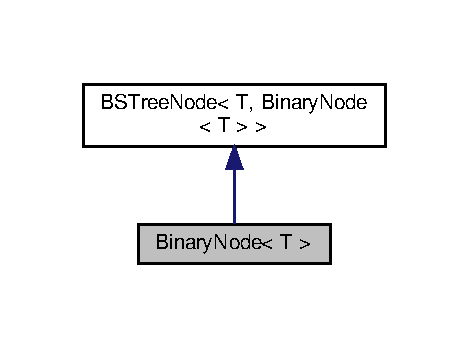
\includegraphics[width=225pt]{classBinaryNode__inherit__graph}
\end{center}
\end{figure}


Collaboration diagram for Binary\+Node$<$ T $>$\+:\nopagebreak
\begin{figure}[H]
\begin{center}
\leavevmode
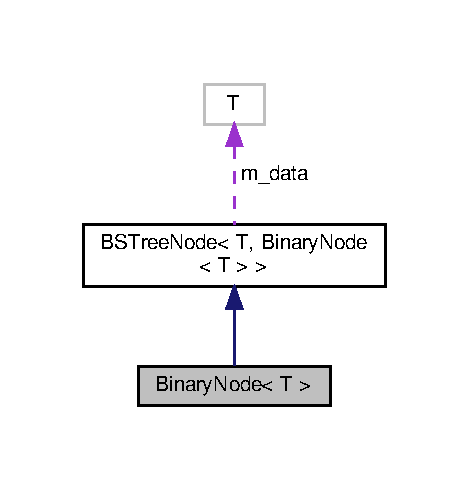
\includegraphics[width=225pt]{classBinaryNode__coll__graph}
\end{center}
\end{figure}
\subsection*{Additional Inherited Members}


\subsection{Detailed Description}
\subsubsection*{template$<$typename T$>$\newline
class Binary\+Node$<$ T $>$}

\subsubsection*{Prédéclarations }

The documentation for this class was generated from the following file\+:\begin{DoxyCompactItemize}
\item 
src/multimap/B\+S\+Tree.\+h\end{DoxyCompactItemize}

\hypertarget{classBSTree}{}\section{B\+S\+Tree$<$ T, N $>$ Class Template Reference}
\label{classBSTree}\index{B\+S\+Tree$<$ T, N $>$@{B\+S\+Tree$<$ T, N $>$}}


Arbre contenant des noeuds génériques.  




{\ttfamily \#include $<$B\+S\+Tree.\+h$>$}

\subsection*{Public Types}
\begin{DoxyCompactItemize}
\item 
using \hyperlink{classBSTree_a9c1a06548b3ff425e1d906f17ce2c858}{Node} = N
\end{DoxyCompactItemize}
\subsection*{Public Member Functions}
\begin{DoxyCompactItemize}
\item 
\hyperlink{classBSTree_a4bdc6f7fed9c195675c2f8b0ebe6fc26}{B\+S\+Tree} ()
\item 
\hyperlink{classBSTree_a9e4b4529c80eea07260e73a0e2d4b448}{B\+S\+Tree} (const \hyperlink{classBSTree}{B\+S\+Tree} \&)=delete
\item 
\hyperlink{classBSTree_a3cc07ee6021bdf3094b2e69cb235eb49}{B\+S\+Tree} (\hyperlink{classBSTree}{B\+S\+Tree} \&\&o)
\item 
\hyperlink{classBSTree_a54457f700c5237425ebb3006b4306cb2}{$\sim$\+B\+S\+Tree} ()
\item 
\hyperlink{classBSTree}{B\+S\+Tree} \& \hyperlink{classBSTree_ac28ab11cb87c12f7338d0f5e1194fb5f}{operator=} (const \hyperlink{classBSTree}{B\+S\+Tree} \&)=delete
\item 
\hyperlink{classBSTree}{B\+S\+Tree} \& \hyperlink{classBSTree_a78c19a61f102ec3999ed62076651b9cb}{operator=} (\hyperlink{classBSTree}{B\+S\+Tree} \&\&o)
\item 
std\+::size\+\_\+t \hyperlink{classBSTree_a5a5453ddeb293754f7a5faf7a11ad066}{size} () const
\item 
bool \hyperlink{classBSTree_a4962f6576d06c47a12a94045b5c1efa8}{empty} () const
\item 
std\+::size\+\_\+t \hyperlink{classBSTree_ad8e76b92cb078260a0e16db55b0ddf00}{height} () const
\item 
\hyperlink{classBSTree_a9c1a06548b3ff425e1d906f17ce2c858}{Node} \& \hyperlink{classBSTree_a079e116466f53f9716387b5ac494f35e}{operator$\ast$} ()
\item 
const \hyperlink{classBSTree_a9c1a06548b3ff425e1d906f17ce2c858}{Node} \& \hyperlink{classBSTree_a59915c35b54e0cef2260759c1392d006}{operator$\ast$} () const
\item 
\hyperlink{classBSTree_a9c1a06548b3ff425e1d906f17ce2c858}{Node} $\ast$ \hyperlink{classBSTree_af16e2ebbb7e4b77039cd4733d0933311}{operator-\/$>$} ()
\item 
const \hyperlink{classBSTree_a9c1a06548b3ff425e1d906f17ce2c858}{Node} $\ast$ \hyperlink{classBSTree_a365c9985b08cb919c11dd91cdc3ef6ac}{operator-\/$>$} () const
\item 
{\footnotesize template$<$typename U $>$ }\\\hyperlink{classBSTree_a9c1a06548b3ff425e1d906f17ce2c858}{Node} $\ast$$\ast$ \hyperlink{classBSTree_ab708b6687e1e241e3b101b5a7d1cff01}{create\+\_\+root} (U \&\&value)
\item 
const \hyperlink{classBSTree_a9c1a06548b3ff425e1d906f17ce2c858}{Node} $\ast$ \hyperlink{classBSTree_a0f3f60e54daa831cb783a922a7e0344c}{root} () const
\item 
\hyperlink{classBSTree_a9c1a06548b3ff425e1d906f17ce2c858}{Node} $\ast$ \hyperlink{classBSTree_aed02cf07356874a6978850a8cf4802aa}{root} ()
\item 
void \hyperlink{classBSTree_a52894175798373289d7e1c779d8ab5f9}{erase} (\hyperlink{classBSTree_a9c1a06548b3ff425e1d906f17ce2c858}{Node} $\ast$node)
\item 
\hyperlink{classBSTree_a9c1a06548b3ff425e1d906f17ce2c858}{Node} $\ast$ \hyperlink{classBSTree_ad43333217921c01d7ea8af358c6b22af}{front} ()
\item 
const \hyperlink{classBSTree_a9c1a06548b3ff425e1d906f17ce2c858}{Node} $\ast$ \hyperlink{classBSTree_a015c11f386bc9f0e8b6ae9351de8daa3}{front} () const
\item 
\hyperlink{classBSTree_a9c1a06548b3ff425e1d906f17ce2c858}{Node} $\ast$ \hyperlink{classBSTree_ae157e3cd6ea405927b214c51578cd999}{back} ()
\item 
const \hyperlink{classBSTree_a9c1a06548b3ff425e1d906f17ce2c858}{Node} $\ast$ \hyperlink{classBSTree_a4089d2fe1ca3ebe90ac7e951dbb50430}{back} () const
\item 
bool \hyperlink{classBSTree_a1228a7a210c99d7986eb74542e189c1f}{equals} (const std\+::initializer\+\_\+list$<$ T $>$ \&initl) const
\item 
bool \hyperlink{classBSTree_aae9d32f9035b1d0aa35a39bf9f196399}{operator!=} (const std\+::initializer\+\_\+list$<$ T $>$ \&initl) const
\item 
bool \hyperlink{classBSTree_a2d4d615e05b62cd917517b0b98150662}{operator==} (const std\+::initializer\+\_\+list$<$ T $>$ \&initl) const
\item 
void \hyperlink{classBSTree_a092be8c378a3f8f5acbd9dfec52d2e87}{clear} ()
\end{DoxyCompactItemize}
\subsection*{Friends}
\begin{DoxyCompactItemize}
\item 
std\+::ostream \& \hyperlink{classBSTree_a1e8a7cc184833a959c0e8139756c22a7}{operator} (std\+::ostream \&lhs, const \hyperlink{classBSTree}{B\+S\+Tree}$<$ T, \hyperlink{classBSTree_a9c1a06548b3ff425e1d906f17ce2c858}{Node} $>$ \&bstree)
\end{DoxyCompactItemize}


\subsection{Detailed Description}
\subsubsection*{template$<$typename T, typename N$>$\newline
class B\+S\+Tree$<$ T, N $>$}

Arbre contenant des noeuds génériques. 

Arbre binaire 
\begin{DoxyTemplParams}{Template Parameters}
{\em T} & type stocké \\
\hline
{\em N} & type du noeud \\
\hline
\end{DoxyTemplParams}


\subsection{Member Typedef Documentation}
\mbox{\Hypertarget{classBSTree_a9c1a06548b3ff425e1d906f17ce2c858}\label{classBSTree_a9c1a06548b3ff425e1d906f17ce2c858}} 
\index{B\+S\+Tree@{B\+S\+Tree}!Node@{Node}}
\index{Node@{Node}!B\+S\+Tree@{B\+S\+Tree}}
\subsubsection{\texorpdfstring{Node}{Node}}
{\footnotesize\ttfamily template$<$typename T, typename N$>$ \\
using \hyperlink{classBSTree}{B\+S\+Tree}$<$ T, N $>$\+::\hyperlink{classBSTree_a9c1a06548b3ff425e1d906f17ce2c858}{Node} =  N}

Type du noeud 

\subsection{Constructor \& Destructor Documentation}
\mbox{\Hypertarget{classBSTree_a4bdc6f7fed9c195675c2f8b0ebe6fc26}\label{classBSTree_a4bdc6f7fed9c195675c2f8b0ebe6fc26}} 
\index{B\+S\+Tree@{B\+S\+Tree}!B\+S\+Tree@{B\+S\+Tree}}
\index{B\+S\+Tree@{B\+S\+Tree}!B\+S\+Tree@{B\+S\+Tree}}
\subsubsection{\texorpdfstring{B\+S\+Tree()}{BSTree()}\hspace{0.1cm}{\footnotesize\ttfamily [1/3]}}
{\footnotesize\ttfamily template$<$typename T, typename N$>$ \\
\hyperlink{classBSTree}{B\+S\+Tree}$<$ T, N $>$\+::\hyperlink{classBSTree}{B\+S\+Tree} (\begin{DoxyParamCaption}{ }\end{DoxyParamCaption})\hspace{0.3cm}{\ttfamily [inline]}}

Constructeur par défaut Créer un arbre vide \mbox{\Hypertarget{classBSTree_a9e4b4529c80eea07260e73a0e2d4b448}\label{classBSTree_a9e4b4529c80eea07260e73a0e2d4b448}} 
\index{B\+S\+Tree@{B\+S\+Tree}!B\+S\+Tree@{B\+S\+Tree}}
\index{B\+S\+Tree@{B\+S\+Tree}!B\+S\+Tree@{B\+S\+Tree}}
\subsubsection{\texorpdfstring{B\+S\+Tree()}{BSTree()}\hspace{0.1cm}{\footnotesize\ttfamily [2/3]}}
{\footnotesize\ttfamily template$<$typename T, typename N$>$ \\
\hyperlink{classBSTree}{B\+S\+Tree}$<$ T, N $>$\+::\hyperlink{classBSTree}{B\+S\+Tree} (\begin{DoxyParamCaption}\item[{const \hyperlink{classBSTree}{B\+S\+Tree}$<$ T, N $>$ \&}]{ }\end{DoxyParamCaption})\hspace{0.3cm}{\ttfamily [delete]}}

Constructeur par copie \mbox{\Hypertarget{classBSTree_a3cc07ee6021bdf3094b2e69cb235eb49}\label{classBSTree_a3cc07ee6021bdf3094b2e69cb235eb49}} 
\index{B\+S\+Tree@{B\+S\+Tree}!B\+S\+Tree@{B\+S\+Tree}}
\index{B\+S\+Tree@{B\+S\+Tree}!B\+S\+Tree@{B\+S\+Tree}}
\subsubsection{\texorpdfstring{B\+S\+Tree()}{BSTree()}\hspace{0.1cm}{\footnotesize\ttfamily [3/3]}}
{\footnotesize\ttfamily template$<$typename T, typename N$>$ \\
\hyperlink{classBSTree}{B\+S\+Tree}$<$ T, N $>$\+::\hyperlink{classBSTree}{B\+S\+Tree} (\begin{DoxyParamCaption}\item[{\hyperlink{classBSTree}{B\+S\+Tree}$<$ T, N $>$ \&\&}]{o }\end{DoxyParamCaption})\hspace{0.3cm}{\ttfamily [inline]}}

Constructeur par déplacement \mbox{\Hypertarget{classBSTree_a54457f700c5237425ebb3006b4306cb2}\label{classBSTree_a54457f700c5237425ebb3006b4306cb2}} 
\index{B\+S\+Tree@{B\+S\+Tree}!````~B\+S\+Tree@{$\sim$\+B\+S\+Tree}}
\index{````~B\+S\+Tree@{$\sim$\+B\+S\+Tree}!B\+S\+Tree@{B\+S\+Tree}}
\subsubsection{\texorpdfstring{$\sim$\+B\+S\+Tree()}{~BSTree()}}
{\footnotesize\ttfamily template$<$typename T, typename N$>$ \\
\hyperlink{classBSTree}{B\+S\+Tree}$<$ T, N $>$\+::$\sim$\hyperlink{classBSTree}{B\+S\+Tree} (\begin{DoxyParamCaption}{ }\end{DoxyParamCaption})\hspace{0.3cm}{\ttfamily [inline]}}

Destructeur 

\subsection{Member Function Documentation}
\mbox{\Hypertarget{classBSTree_ae157e3cd6ea405927b214c51578cd999}\label{classBSTree_ae157e3cd6ea405927b214c51578cd999}} 
\index{B\+S\+Tree@{B\+S\+Tree}!back@{back}}
\index{back@{back}!B\+S\+Tree@{B\+S\+Tree}}
\subsubsection{\texorpdfstring{back()}{back()}\hspace{0.1cm}{\footnotesize\ttfamily [1/2]}}
{\footnotesize\ttfamily template$<$typename T, typename N$>$ \\
\hyperlink{classBSTree_a9c1a06548b3ff425e1d906f17ce2c858}{Node}$\ast$ \hyperlink{classBSTree}{B\+S\+Tree}$<$ T, N $>$\+::back (\begin{DoxyParamCaption}{ }\end{DoxyParamCaption})\hspace{0.3cm}{\ttfamily [inline]}}

Récupérer l\textquotesingle{}élément le plus grand de l\textquotesingle{}arbre (non constant) L\textquotesingle{}arbre ne doit pas être vide \mbox{\Hypertarget{classBSTree_a4089d2fe1ca3ebe90ac7e951dbb50430}\label{classBSTree_a4089d2fe1ca3ebe90ac7e951dbb50430}} 
\index{B\+S\+Tree@{B\+S\+Tree}!back@{back}}
\index{back@{back}!B\+S\+Tree@{B\+S\+Tree}}
\subsubsection{\texorpdfstring{back()}{back()}\hspace{0.1cm}{\footnotesize\ttfamily [2/2]}}
{\footnotesize\ttfamily template$<$typename T, typename N$>$ \\
const \hyperlink{classBSTree_a9c1a06548b3ff425e1d906f17ce2c858}{Node}$\ast$ \hyperlink{classBSTree}{B\+S\+Tree}$<$ T, N $>$\+::back (\begin{DoxyParamCaption}{ }\end{DoxyParamCaption}) const\hspace{0.3cm}{\ttfamily [inline]}}

Récupérer l\textquotesingle{}élément le plus petit de l\textquotesingle{}arbre (constant) L\textquotesingle{}arbre ne doit pas être vide \mbox{\Hypertarget{classBSTree_a092be8c378a3f8f5acbd9dfec52d2e87}\label{classBSTree_a092be8c378a3f8f5acbd9dfec52d2e87}} 
\index{B\+S\+Tree@{B\+S\+Tree}!clear@{clear}}
\index{clear@{clear}!B\+S\+Tree@{B\+S\+Tree}}
\subsubsection{\texorpdfstring{clear()}{clear()}}
{\footnotesize\ttfamily template$<$typename T, typename N$>$ \\
void \hyperlink{classBSTree}{B\+S\+Tree}$<$ T, N $>$\+::clear (\begin{DoxyParamCaption}{ }\end{DoxyParamCaption})\hspace{0.3cm}{\ttfamily [inline]}}

Vider entièrement l\textquotesingle{}arbre. Si l\textquotesingle{}arbre était déjà vide, ne fait rien. \mbox{\Hypertarget{classBSTree_ab708b6687e1e241e3b101b5a7d1cff01}\label{classBSTree_ab708b6687e1e241e3b101b5a7d1cff01}} 
\index{B\+S\+Tree@{B\+S\+Tree}!create\+\_\+root@{create\+\_\+root}}
\index{create\+\_\+root@{create\+\_\+root}!B\+S\+Tree@{B\+S\+Tree}}
\subsubsection{\texorpdfstring{create\+\_\+root()}{create\_root()}}
{\footnotesize\ttfamily template$<$typename T, typename N$>$ \\
template$<$typename U $>$ \\
\hyperlink{classBSTree_a9c1a06548b3ff425e1d906f17ce2c858}{Node}$\ast$$\ast$ \hyperlink{classBSTree}{B\+S\+Tree}$<$ T, N $>$\+::create\+\_\+root (\begin{DoxyParamCaption}\item[{U \&\&}]{value }\end{DoxyParamCaption})\hspace{0.3cm}{\ttfamily [inline]}}

Créer une racine par référence universelle (copie ou déplacement). L\textquotesingle{}arbre doit être vide. 
\begin{DoxyParams}{Parameters}
{\em value} & La valeur de la racine \\
\hline
\end{DoxyParams}
\mbox{\Hypertarget{classBSTree_a4962f6576d06c47a12a94045b5c1efa8}\label{classBSTree_a4962f6576d06c47a12a94045b5c1efa8}} 
\index{B\+S\+Tree@{B\+S\+Tree}!empty@{empty}}
\index{empty@{empty}!B\+S\+Tree@{B\+S\+Tree}}
\subsubsection{\texorpdfstring{empty()}{empty()}}
{\footnotesize\ttfamily template$<$typename T, typename N$>$ \\
bool \hyperlink{classBSTree}{B\+S\+Tree}$<$ T, N $>$\+::empty (\begin{DoxyParamCaption}{ }\end{DoxyParamCaption}) const\hspace{0.3cm}{\ttfamily [inline]}}

Tester si l\textquotesingle{}arbre est vide (c\textquotesingle{}est-\/à-\/dire s\textquotesingle{}il contient 0 noeuds).

\begin{DoxyReturn}{Returns}
true si l\textquotesingle{}arbre est vide, false sinon 
\end{DoxyReturn}
\mbox{\Hypertarget{classBSTree_a1228a7a210c99d7986eb74542e189c1f}\label{classBSTree_a1228a7a210c99d7986eb74542e189c1f}} 
\index{B\+S\+Tree@{B\+S\+Tree}!equals@{equals}}
\index{equals@{equals}!B\+S\+Tree@{B\+S\+Tree}}
\subsubsection{\texorpdfstring{equals()}{equals()}}
{\footnotesize\ttfamily template$<$typename T, typename N$>$ \\
bool \hyperlink{classBSTree}{B\+S\+Tree}$<$ T, N $>$\+::equals (\begin{DoxyParamCaption}\item[{const std\+::initializer\+\_\+list$<$ T $>$ \&}]{initl }\end{DoxyParamCaption}) const\hspace{0.3cm}{\ttfamily [inline]}}

Comparaison avec une liste d\textquotesingle{}initialisation. Fournit une méthode \hyperlink{classBSTree_a1228a7a210c99d7986eb74542e189c1f}{equals()} car on ne peut pas comparer directement une liste d\textquotesingle{}initialisation littérale avec l\textquotesingle{}opérateur ==.


\begin{DoxyParams}{Parameters}
{\em initl} & la liste d\textquotesingle{}initialisation à comparer\\
\hline
\end{DoxyParams}
\begin{DoxyReturn}{Returns}
true si la liste d\textquotesingle{}initialisation correspond à l\textquotesingle{}arbre dans l\textquotesingle{}ordre infixe, false sinon. 
\end{DoxyReturn}
\mbox{\Hypertarget{classBSTree_a52894175798373289d7e1c779d8ab5f9}\label{classBSTree_a52894175798373289d7e1c779d8ab5f9}} 
\index{B\+S\+Tree@{B\+S\+Tree}!erase@{erase}}
\index{erase@{erase}!B\+S\+Tree@{B\+S\+Tree}}
\subsubsection{\texorpdfstring{erase()}{erase()}}
{\footnotesize\ttfamily template$<$typename T, typename N$>$ \\
void \hyperlink{classBSTree}{B\+S\+Tree}$<$ T, N $>$\+::erase (\begin{DoxyParamCaption}\item[{\hyperlink{classBSTree_a9c1a06548b3ff425e1d906f17ce2c858}{Node} $\ast$}]{node }\end{DoxyParamCaption})\hspace{0.3cm}{\ttfamily [inline]}}

Supprime un noeud de l\textquotesingle{}arbre L\textquotesingle{}arbre ne doit pas être vide


\begin{DoxyParams}{Parameters}
{\em node} & le noeud à supprimer \\
\hline
\end{DoxyParams}
Insérer le noeud \mbox{\Hypertarget{classBSTree_ad43333217921c01d7ea8af358c6b22af}\label{classBSTree_ad43333217921c01d7ea8af358c6b22af}} 
\index{B\+S\+Tree@{B\+S\+Tree}!front@{front}}
\index{front@{front}!B\+S\+Tree@{B\+S\+Tree}}
\subsubsection{\texorpdfstring{front()}{front()}\hspace{0.1cm}{\footnotesize\ttfamily [1/2]}}
{\footnotesize\ttfamily template$<$typename T, typename N$>$ \\
\hyperlink{classBSTree_a9c1a06548b3ff425e1d906f17ce2c858}{Node}$\ast$ \hyperlink{classBSTree}{B\+S\+Tree}$<$ T, N $>$\+::front (\begin{DoxyParamCaption}{ }\end{DoxyParamCaption})\hspace{0.3cm}{\ttfamily [inline]}}

Récupérer l\textquotesingle{}élément le plus petit de l\textquotesingle{}arbre (non constant) L\textquotesingle{}arbre ne doit pas être vide \mbox{\Hypertarget{classBSTree_a015c11f386bc9f0e8b6ae9351de8daa3}\label{classBSTree_a015c11f386bc9f0e8b6ae9351de8daa3}} 
\index{B\+S\+Tree@{B\+S\+Tree}!front@{front}}
\index{front@{front}!B\+S\+Tree@{B\+S\+Tree}}
\subsubsection{\texorpdfstring{front()}{front()}\hspace{0.1cm}{\footnotesize\ttfamily [2/2]}}
{\footnotesize\ttfamily template$<$typename T, typename N$>$ \\
const \hyperlink{classBSTree_a9c1a06548b3ff425e1d906f17ce2c858}{Node}$\ast$ \hyperlink{classBSTree}{B\+S\+Tree}$<$ T, N $>$\+::front (\begin{DoxyParamCaption}{ }\end{DoxyParamCaption}) const\hspace{0.3cm}{\ttfamily [inline]}}

Récupérer l\textquotesingle{}élément le plus petit de l\textquotesingle{}arbre (constant) L\textquotesingle{}arbre ne doit pas être vide \mbox{\Hypertarget{classBSTree_ad8e76b92cb078260a0e16db55b0ddf00}\label{classBSTree_ad8e76b92cb078260a0e16db55b0ddf00}} 
\index{B\+S\+Tree@{B\+S\+Tree}!height@{height}}
\index{height@{height}!B\+S\+Tree@{B\+S\+Tree}}
\subsubsection{\texorpdfstring{height()}{height()}}
{\footnotesize\ttfamily template$<$typename T, typename N$>$ \\
std\+::size\+\_\+t \hyperlink{classBSTree}{B\+S\+Tree}$<$ T, N $>$\+::height (\begin{DoxyParamCaption}{ }\end{DoxyParamCaption}) const\hspace{0.3cm}{\ttfamily [inline]}}

Récupère la hauteur de l\textquotesingle{}arbre (récursif)

\begin{DoxyReturn}{Returns}
la hauteur de l\textquotesingle{}arbre. 0 si l\textquotesingle{}arbre est vide 
\end{DoxyReturn}
\mbox{\Hypertarget{classBSTree_aae9d32f9035b1d0aa35a39bf9f196399}\label{classBSTree_aae9d32f9035b1d0aa35a39bf9f196399}} 
\index{B\+S\+Tree@{B\+S\+Tree}!operator"!=@{operator"!=}}
\index{operator"!=@{operator"!=}!B\+S\+Tree@{B\+S\+Tree}}
\subsubsection{\texorpdfstring{operator"!=()}{operator!=()}}
{\footnotesize\ttfamily template$<$typename T, typename N$>$ \\
bool \hyperlink{classBSTree}{B\+S\+Tree}$<$ T, N $>$\+::operator!= (\begin{DoxyParamCaption}\item[{const std\+::initializer\+\_\+list$<$ T $>$ \&}]{initl }\end{DoxyParamCaption}) const\hspace{0.3cm}{\ttfamily [inline]}}

Comparaison avec une liste d\textquotesingle{}initialisation


\begin{DoxyParams}{Parameters}
{\em initl} & la liste d\textquotesingle{}initialisation à comparer\\
\hline
\end{DoxyParams}
\begin{DoxyReturn}{Returns}
false si la liste d\textquotesingle{}initialisation correspond à l\textquotesingle{}arbre dans l\textquotesingle{}ordre infixe, true sinon. 
\end{DoxyReturn}
\mbox{\Hypertarget{classBSTree_a079e116466f53f9716387b5ac494f35e}\label{classBSTree_a079e116466f53f9716387b5ac494f35e}} 
\index{B\+S\+Tree@{B\+S\+Tree}!operator$\ast$@{operator$\ast$}}
\index{operator$\ast$@{operator$\ast$}!B\+S\+Tree@{B\+S\+Tree}}
\subsubsection{\texorpdfstring{operator$\ast$()}{operator*()}\hspace{0.1cm}{\footnotesize\ttfamily [1/2]}}
{\footnotesize\ttfamily template$<$typename T, typename N$>$ \\
\hyperlink{classBSTree_a9c1a06548b3ff425e1d906f17ce2c858}{Node}\& \hyperlink{classBSTree}{B\+S\+Tree}$<$ T, N $>$\+::\hyperlink{classBSTree_a1e8a7cc184833a959c0e8139756c22a7}{operator}$\ast$ (\begin{DoxyParamCaption}{ }\end{DoxyParamCaption})\hspace{0.3cm}{\ttfamily [inline]}}

Récupération des données (non constant) \mbox{\Hypertarget{classBSTree_a59915c35b54e0cef2260759c1392d006}\label{classBSTree_a59915c35b54e0cef2260759c1392d006}} 
\index{B\+S\+Tree@{B\+S\+Tree}!operator$\ast$@{operator$\ast$}}
\index{operator$\ast$@{operator$\ast$}!B\+S\+Tree@{B\+S\+Tree}}
\subsubsection{\texorpdfstring{operator$\ast$()}{operator*()}\hspace{0.1cm}{\footnotesize\ttfamily [2/2]}}
{\footnotesize\ttfamily template$<$typename T, typename N$>$ \\
const \hyperlink{classBSTree_a9c1a06548b3ff425e1d906f17ce2c858}{Node}\& \hyperlink{classBSTree}{B\+S\+Tree}$<$ T, N $>$\+::\hyperlink{classBSTree_a1e8a7cc184833a959c0e8139756c22a7}{operator}$\ast$ (\begin{DoxyParamCaption}{ }\end{DoxyParamCaption}) const\hspace{0.3cm}{\ttfamily [inline]}}

Récupération des données (constant) \mbox{\Hypertarget{classBSTree_af16e2ebbb7e4b77039cd4733d0933311}\label{classBSTree_af16e2ebbb7e4b77039cd4733d0933311}} 
\index{B\+S\+Tree@{B\+S\+Tree}!operator-\/$>$@{operator-\/$>$}}
\index{operator-\/$>$@{operator-\/$>$}!B\+S\+Tree@{B\+S\+Tree}}
\subsubsection{\texorpdfstring{operator-\/$>$()}{operator->()}\hspace{0.1cm}{\footnotesize\ttfamily [1/2]}}
{\footnotesize\ttfamily template$<$typename T, typename N$>$ \\
\hyperlink{classBSTree_a9c1a06548b3ff425e1d906f17ce2c858}{Node}$\ast$ \hyperlink{classBSTree}{B\+S\+Tree}$<$ T, N $>$\+::\hyperlink{classBSTree_a1e8a7cc184833a959c0e8139756c22a7}{operator}-\/$>$ (\begin{DoxyParamCaption}{ }\end{DoxyParamCaption})\hspace{0.3cm}{\ttfamily [inline]}}

Récupération des données pointées (non constant) \mbox{\Hypertarget{classBSTree_a365c9985b08cb919c11dd91cdc3ef6ac}\label{classBSTree_a365c9985b08cb919c11dd91cdc3ef6ac}} 
\index{B\+S\+Tree@{B\+S\+Tree}!operator-\/$>$@{operator-\/$>$}}
\index{operator-\/$>$@{operator-\/$>$}!B\+S\+Tree@{B\+S\+Tree}}
\subsubsection{\texorpdfstring{operator-\/$>$()}{operator->()}\hspace{0.1cm}{\footnotesize\ttfamily [2/2]}}
{\footnotesize\ttfamily template$<$typename T, typename N$>$ \\
const \hyperlink{classBSTree_a9c1a06548b3ff425e1d906f17ce2c858}{Node}$\ast$ \hyperlink{classBSTree}{B\+S\+Tree}$<$ T, N $>$\+::\hyperlink{classBSTree_a1e8a7cc184833a959c0e8139756c22a7}{operator}-\/$>$ (\begin{DoxyParamCaption}{ }\end{DoxyParamCaption}) const\hspace{0.3cm}{\ttfamily [inline]}}

Récupération des données pointées (constant) \mbox{\Hypertarget{classBSTree_ac28ab11cb87c12f7338d0f5e1194fb5f}\label{classBSTree_ac28ab11cb87c12f7338d0f5e1194fb5f}} 
\index{B\+S\+Tree@{B\+S\+Tree}!operator=@{operator=}}
\index{operator=@{operator=}!B\+S\+Tree@{B\+S\+Tree}}
\subsubsection{\texorpdfstring{operator=()}{operator=()}\hspace{0.1cm}{\footnotesize\ttfamily [1/2]}}
{\footnotesize\ttfamily template$<$typename T, typename N$>$ \\
\hyperlink{classBSTree}{B\+S\+Tree}\& \hyperlink{classBSTree}{B\+S\+Tree}$<$ T, N $>$\+::\hyperlink{classBSTree_a1e8a7cc184833a959c0e8139756c22a7}{operator}= (\begin{DoxyParamCaption}\item[{const \hyperlink{classBSTree}{B\+S\+Tree}$<$ T, N $>$ \&}]{ }\end{DoxyParamCaption})\hspace{0.3cm}{\ttfamily [delete]}}

Assignation par copie \mbox{\Hypertarget{classBSTree_a78c19a61f102ec3999ed62076651b9cb}\label{classBSTree_a78c19a61f102ec3999ed62076651b9cb}} 
\index{B\+S\+Tree@{B\+S\+Tree}!operator=@{operator=}}
\index{operator=@{operator=}!B\+S\+Tree@{B\+S\+Tree}}
\subsubsection{\texorpdfstring{operator=()}{operator=()}\hspace{0.1cm}{\footnotesize\ttfamily [2/2]}}
{\footnotesize\ttfamily template$<$typename T, typename N$>$ \\
\hyperlink{classBSTree}{B\+S\+Tree}\& \hyperlink{classBSTree}{B\+S\+Tree}$<$ T, N $>$\+::\hyperlink{classBSTree_a1e8a7cc184833a959c0e8139756c22a7}{operator}= (\begin{DoxyParamCaption}\item[{\hyperlink{classBSTree}{B\+S\+Tree}$<$ T, N $>$ \&\&}]{o }\end{DoxyParamCaption})\hspace{0.3cm}{\ttfamily [inline]}}

Assignation par déplacement \mbox{\Hypertarget{classBSTree_a2d4d615e05b62cd917517b0b98150662}\label{classBSTree_a2d4d615e05b62cd917517b0b98150662}} 
\index{B\+S\+Tree@{B\+S\+Tree}!operator==@{operator==}}
\index{operator==@{operator==}!B\+S\+Tree@{B\+S\+Tree}}
\subsubsection{\texorpdfstring{operator==()}{operator==()}}
{\footnotesize\ttfamily template$<$typename T, typename N$>$ \\
bool \hyperlink{classBSTree}{B\+S\+Tree}$<$ T, N $>$\+::\hyperlink{classBSTree_a1e8a7cc184833a959c0e8139756c22a7}{operator}== (\begin{DoxyParamCaption}\item[{const std\+::initializer\+\_\+list$<$ T $>$ \&}]{initl }\end{DoxyParamCaption}) const\hspace{0.3cm}{\ttfamily [inline]}}

Comparaison avec une liste d\textquotesingle{}initialisation.


\begin{DoxyParams}{Parameters}
{\em initl} & la liste d\textquotesingle{}initialisation à comparer\\
\hline
\end{DoxyParams}
\begin{DoxyReturn}{Returns}
true si la liste d\textquotesingle{}initialisation correspond à l\textquotesingle{}arbre dans l\textquotesingle{}ordre infixe, false sinon. 
\end{DoxyReturn}
\mbox{\Hypertarget{classBSTree_a0f3f60e54daa831cb783a922a7e0344c}\label{classBSTree_a0f3f60e54daa831cb783a922a7e0344c}} 
\index{B\+S\+Tree@{B\+S\+Tree}!root@{root}}
\index{root@{root}!B\+S\+Tree@{B\+S\+Tree}}
\subsubsection{\texorpdfstring{root()}{root()}\hspace{0.1cm}{\footnotesize\ttfamily [1/2]}}
{\footnotesize\ttfamily template$<$typename T, typename N$>$ \\
const \hyperlink{classBSTree_a9c1a06548b3ff425e1d906f17ce2c858}{Node}$\ast$ \hyperlink{classBSTree}{B\+S\+Tree}$<$ T, N $>$\+::root (\begin{DoxyParamCaption}{ }\end{DoxyParamCaption}) const\hspace{0.3cm}{\ttfamily [inline]}}

Récupère la racine de l\textquotesingle{}arbre (constant) L\textquotesingle{}arbre ne doit pas être vide \mbox{\Hypertarget{classBSTree_aed02cf07356874a6978850a8cf4802aa}\label{classBSTree_aed02cf07356874a6978850a8cf4802aa}} 
\index{B\+S\+Tree@{B\+S\+Tree}!root@{root}}
\index{root@{root}!B\+S\+Tree@{B\+S\+Tree}}
\subsubsection{\texorpdfstring{root()}{root()}\hspace{0.1cm}{\footnotesize\ttfamily [2/2]}}
{\footnotesize\ttfamily template$<$typename T, typename N$>$ \\
\hyperlink{classBSTree_a9c1a06548b3ff425e1d906f17ce2c858}{Node}$\ast$ \hyperlink{classBSTree}{B\+S\+Tree}$<$ T, N $>$\+::root (\begin{DoxyParamCaption}{ }\end{DoxyParamCaption})\hspace{0.3cm}{\ttfamily [inline]}}

Récupère la racine de l\textquotesingle{}arbre (non constant) L\textquotesingle{}arbre ne doit pas être vide \mbox{\Hypertarget{classBSTree_a5a5453ddeb293754f7a5faf7a11ad066}\label{classBSTree_a5a5453ddeb293754f7a5faf7a11ad066}} 
\index{B\+S\+Tree@{B\+S\+Tree}!size@{size}}
\index{size@{size}!B\+S\+Tree@{B\+S\+Tree}}
\subsubsection{\texorpdfstring{size()}{size()}}
{\footnotesize\ttfamily template$<$typename T, typename N$>$ \\
std\+::size\+\_\+t \hyperlink{classBSTree}{B\+S\+Tree}$<$ T, N $>$\+::size (\begin{DoxyParamCaption}{ }\end{DoxyParamCaption}) const\hspace{0.3cm}{\ttfamily [inline]}}

Récupère la taille de l\textquotesingle{}arbre (récursif)

\begin{DoxyReturn}{Returns}
le nombre de noeuds de l\textquotesingle{}arbre 
\end{DoxyReturn}


\subsection{Friends And Related Function Documentation}
\mbox{\Hypertarget{classBSTree_a1e8a7cc184833a959c0e8139756c22a7}\label{classBSTree_a1e8a7cc184833a959c0e8139756c22a7}} 
\index{B\+S\+Tree@{B\+S\+Tree}!operator@{operator}}
\index{operator@{operator}!B\+S\+Tree@{B\+S\+Tree}}
\subsubsection{\texorpdfstring{operator}{operator}}
{\footnotesize\ttfamily template$<$typename T, typename N$>$ \\
std\+::ostream\& operator (\begin{DoxyParamCaption}\item[{std\+::ostream \&}]{lhs,  }\item[{const \hyperlink{classBSTree}{B\+S\+Tree}$<$ T, \hyperlink{classBSTree_a9c1a06548b3ff425e1d906f17ce2c858}{Node} $>$ \&}]{bstree }\end{DoxyParamCaption})\hspace{0.3cm}{\ttfamily [friend]}}

Affichage de l\textquotesingle{}arbre dans un flux (en infixé, ou sous forme d\textquotesingle{}arbre) 

The documentation for this class was generated from the following file\+:\begin{DoxyCompactItemize}
\item 
src/multimap/B\+S\+Tree.\+h\end{DoxyCompactItemize}

\hypertarget{classBSTreeNode}{}\section{B\+S\+Tree\+Node$<$ T, Node $>$ Class Template Reference}
\label{classBSTreeNode}\index{B\+S\+Tree\+Node$<$ T, Node $>$@{B\+S\+Tree\+Node$<$ T, Node $>$}}


{\ttfamily \#include $<$B\+S\+Tree.\+h$>$}



Collaboration diagram for B\+S\+Tree\+Node$<$ T, Node $>$\+:\nopagebreak
\begin{figure}[H]
\begin{center}
\leavevmode
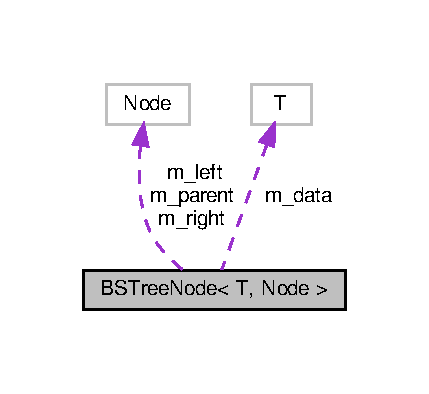
\includegraphics[width=206pt]{classBSTreeNode__coll__graph}
\end{center}
\end{figure}
\subsection*{Public Member Functions}
\begin{DoxyCompactItemize}
\item 
\mbox{\Hypertarget{classBSTreeNode_a38185eb6c1f1e481ccf9c9be63c0d7be}\label{classBSTreeNode_a38185eb6c1f1e481ccf9c9be63c0d7be}} 
std\+::size\+\_\+t {\bfseries size} () const
\item 
\mbox{\Hypertarget{classBSTreeNode_a152a91576afe7e3da0326ae28bb582a7}\label{classBSTreeNode_a152a91576afe7e3da0326ae28bb582a7}} 
bool \hyperlink{classBSTreeNode_a152a91576afe7e3da0326ae28bb582a7}{is\+\_\+root} () const
\begin{DoxyCompactList}\small\item\em Retourne vrai si le noeud est la racine, faux sinon. \end{DoxyCompactList}\item 
\mbox{\Hypertarget{classBSTreeNode_aca5df2aae136860532a39e160269e266}\label{classBSTreeNode_aca5df2aae136860532a39e160269e266}} 
bool \hyperlink{classBSTreeNode_aca5df2aae136860532a39e160269e266}{is\+\_\+leaf} () const
\begin{DoxyCompactList}\small\item\em Retourne vrai si le noeud est une feuille, faux sinon. \end{DoxyCompactList}\item 
\mbox{\Hypertarget{classBSTreeNode_a8a25ff9fcd33464ba3ef8b9ef9c09203}\label{classBSTreeNode_a8a25ff9fcd33464ba3ef8b9ef9c09203}} 
bool \hyperlink{classBSTreeNode_a8a25ff9fcd33464ba3ef8b9ef9c09203}{has\+\_\+left} () const
\begin{DoxyCompactList}\small\item\em Retourne vrai si le noeud a un fils gauche. \end{DoxyCompactList}\item 
\mbox{\Hypertarget{classBSTreeNode_aa73c6b24891bac61df942c99d2b689bd}\label{classBSTreeNode_aa73c6b24891bac61df942c99d2b689bd}} 
bool \hyperlink{classBSTreeNode_aa73c6b24891bac61df942c99d2b689bd}{has\+\_\+right} () const
\begin{DoxyCompactList}\small\item\em Retourne vrai si le noeud a un fils droit. \end{DoxyCompactList}\item 
\mbox{\Hypertarget{classBSTreeNode_a74a9baf20cf5ae5bf40ca83a5a611db9}\label{classBSTreeNode_a74a9baf20cf5ae5bf40ca83a5a611db9}} 
const T \& \hyperlink{classBSTreeNode_a74a9baf20cf5ae5bf40ca83a5a611db9}{data} () const
\begin{DoxyCompactList}\small\item\em Récupère la donnée (constant) \end{DoxyCompactList}\item 
\mbox{\Hypertarget{classBSTreeNode_adab11a903f0e299e736a3fb29fb8dead}\label{classBSTreeNode_adab11a903f0e299e736a3fb29fb8dead}} 
T \& \hyperlink{classBSTreeNode_adab11a903f0e299e736a3fb29fb8dead}{data} ()
\begin{DoxyCompactList}\small\item\em Récupère la donnée (non-\/constant) \end{DoxyCompactList}\item 
\mbox{\Hypertarget{classBSTreeNode_aa1a36ab9699282b3b0b665951735a387}\label{classBSTreeNode_aa1a36ab9699282b3b0b665951735a387}} 
const Node $\ast$ \hyperlink{classBSTreeNode_aa1a36ab9699282b3b0b665951735a387}{parent} () const
\begin{DoxyCompactList}\small\item\em Récupère le parent du noeud courant (constant) \end{DoxyCompactList}\item 
\mbox{\Hypertarget{classBSTreeNode_a331cbf0e1756db6a3f0ec0e4c5288aba}\label{classBSTreeNode_a331cbf0e1756db6a3f0ec0e4c5288aba}} 
Node $\ast$ \hyperlink{classBSTreeNode_a331cbf0e1756db6a3f0ec0e4c5288aba}{parent} ()
\begin{DoxyCompactList}\small\item\em Récupère le parent du noeud courant (non-\/constant) \end{DoxyCompactList}\item 
\mbox{\Hypertarget{classBSTreeNode_a0167920e3e97c4f41900482c2c02145e}\label{classBSTreeNode_a0167920e3e97c4f41900482c2c02145e}} 
const Node $\ast$ \hyperlink{classBSTreeNode_a0167920e3e97c4f41900482c2c02145e}{left} () const
\begin{DoxyCompactList}\small\item\em Récupère le fils gauche (constant) \end{DoxyCompactList}\item 
\mbox{\Hypertarget{classBSTreeNode_a4561562eb320ae7ab88f9edb7b872022}\label{classBSTreeNode_a4561562eb320ae7ab88f9edb7b872022}} 
Node $\ast$ \hyperlink{classBSTreeNode_a4561562eb320ae7ab88f9edb7b872022}{left} ()
\begin{DoxyCompactList}\small\item\em Récupère le fils gauche (non-\/constant) \end{DoxyCompactList}\item 
\mbox{\Hypertarget{classBSTreeNode_a791628dcbe4d70541227882b42592d1f}\label{classBSTreeNode_a791628dcbe4d70541227882b42592d1f}} 
const Node $\ast$ \hyperlink{classBSTreeNode_a791628dcbe4d70541227882b42592d1f}{right} () const
\begin{DoxyCompactList}\small\item\em Récupère le fils droit (constant) \end{DoxyCompactList}\item 
\mbox{\Hypertarget{classBSTreeNode_aa4f11b0043d113545c1a407a844939ee}\label{classBSTreeNode_aa4f11b0043d113545c1a407a844939ee}} 
Node $\ast$ \hyperlink{classBSTreeNode_aa4f11b0043d113545c1a407a844939ee}{right} ()
\begin{DoxyCompactList}\small\item\em Récupère le fils droit (non-\/constant) \end{DoxyCompactList}\item 
\mbox{\Hypertarget{classBSTreeNode_aea220a44e4c4f9a835d03d75b6851a56}\label{classBSTreeNode_aea220a44e4c4f9a835d03d75b6851a56}} 
std\+::size\+\_\+t \hyperlink{classBSTreeNode_aea220a44e4c4f9a835d03d75b6851a56}{height} () const
\begin{DoxyCompactList}\small\item\em Hauteur du noeud. \end{DoxyCompactList}\item 
Node $\ast$ \hyperlink{classBSTreeNode_aa2bc109220f6782ad1f9fbb80b7dca60}{max} ()
\item 
Node $\ast$ \hyperlink{classBSTreeNode_a02645620a3cb4ab4f9d15b1207422cb3}{min} ()
\item 
\mbox{\Hypertarget{classBSTreeNode_a2a4500849e93739a886fa6dd011fff4b}\label{classBSTreeNode_a2a4500849e93739a886fa6dd011fff4b}} 
Node $\ast$ \hyperlink{classBSTreeNode_a2a4500849e93739a886fa6dd011fff4b}{next} ()
\begin{DoxyCompactList}\small\item\em Récupère le noeud suivant (ou N\+U\+LL si c\textquotesingle{}est le dernier noeud) \end{DoxyCompactList}\item 
\mbox{\Hypertarget{classBSTreeNode_ad9cb1ab6bc14396ce1ed8405fb996352}\label{classBSTreeNode_ad9cb1ab6bc14396ce1ed8405fb996352}} 
const Node $\ast$ {\bfseries next} () const
\item 
\mbox{\Hypertarget{classBSTreeNode_a6a51620ecd4f94569c128d3d2f7608cc}\label{classBSTreeNode_a6a51620ecd4f94569c128d3d2f7608cc}} 
Node $\ast$ \hyperlink{classBSTreeNode_a6a51620ecd4f94569c128d3d2f7608cc}{prev} ()
\begin{DoxyCompactList}\small\item\em Récupère le noeud précédent (ou N\+U\+LL si c\textquotesingle{}est le premier noeud) \end{DoxyCompactList}\item 
\mbox{\Hypertarget{classBSTreeNode_a8fdc7c579693763ee554b2a7c3ff34a3}\label{classBSTreeNode_a8fdc7c579693763ee554b2a7c3ff34a3}} 
const Node $\ast$ {\bfseries prev} () const
\item 
\mbox{\Hypertarget{classBSTreeNode_a85987179fb53e998efa895d3b181916c}\label{classBSTreeNode_a85987179fb53e998efa895d3b181916c}} 
{\footnotesize template$<$typename U $>$ }\\Node $\ast$ \hyperlink{classBSTreeNode_a85987179fb53e998efa895d3b181916c}{insert\+\_\+left} (U \&\&t)
\begin{DoxyCompactList}\small\item\em Insère un noeud à gauche. \end{DoxyCompactList}\item 
\mbox{\Hypertarget{classBSTreeNode_a6048387f72db53ce0ed8567a570c468e}\label{classBSTreeNode_a6048387f72db53ce0ed8567a570c468e}} 
{\footnotesize template$<$typename U $>$ }\\Node $\ast$ \hyperlink{classBSTreeNode_a6048387f72db53ce0ed8567a570c468e}{insert\+\_\+right} (U \&\&t)
\begin{DoxyCompactList}\small\item\em Insère un noeud à droite. \end{DoxyCompactList}\end{DoxyCompactItemize}
\subsection*{Protected Member Functions}
\begin{DoxyCompactItemize}
\item 
\mbox{\Hypertarget{classBSTreeNode_ac25c7c68f27e3372510d4ebf3caf920c}\label{classBSTreeNode_ac25c7c68f27e3372510d4ebf3caf920c}} 
{\footnotesize template$<$typename U $>$ }\\{\bfseries B\+S\+Tree\+Node} (U \&\&t, Node $\ast$parent\+Node=nullptr)
\item 
\mbox{\Hypertarget{classBSTreeNode_a8e95ffc728076e81c1bbccfeb47a26f7}\label{classBSTreeNode_a8e95ffc728076e81c1bbccfeb47a26f7}} 
void {\bfseries deep\+Erase\+Children} ()
\item 
\mbox{\Hypertarget{classBSTreeNode_a128a6509a2779f97a83b91cf3c9ed6b0}\label{classBSTreeNode_a128a6509a2779f97a83b91cf3c9ed6b0}} 
void {\bfseries replace\+Child} (Node $\ast$old\+Child, Node $\ast$new\+Child)
\end{DoxyCompactItemize}
\subsection*{Protected Attributes}
\begin{DoxyCompactItemize}
\item 
\mbox{\Hypertarget{classBSTreeNode_a90e1d54d52717e3fe774178a05d46b85}\label{classBSTreeNode_a90e1d54d52717e3fe774178a05d46b85}} 
T $\ast$ {\bfseries m\+\_\+data}
\item 
\mbox{\Hypertarget{classBSTreeNode_a44da72e439fe5ced0255f09bfd2d05b4}\label{classBSTreeNode_a44da72e439fe5ced0255f09bfd2d05b4}} 
Node $\ast$ {\bfseries m\+\_\+parent}
\item 
\mbox{\Hypertarget{classBSTreeNode_a5fe5a7c75b5f4d5dc3f853d1c1b2e7e1}\label{classBSTreeNode_a5fe5a7c75b5f4d5dc3f853d1c1b2e7e1}} 
Node $\ast$ {\bfseries m\+\_\+left}
\item 
\mbox{\Hypertarget{classBSTreeNode_a3e9c2232d64f5ba0a1e77782832ada3a}\label{classBSTreeNode_a3e9c2232d64f5ba0a1e77782832ada3a}} 
Node $\ast$ {\bfseries m\+\_\+right}
\end{DoxyCompactItemize}
\subsection*{Friends}
\begin{DoxyCompactItemize}
\item 
\mbox{\Hypertarget{classBSTreeNode_a73f30f7d205b76caf0f18c05ea1ee795}\label{classBSTreeNode_a73f30f7d205b76caf0f18c05ea1ee795}} 
class {\bfseries B\+S\+Tree$<$ T, Node $>$}
\item 
\mbox{\Hypertarget{classBSTreeNode_a1e8a7cc184833a959c0e8139756c22a7}\label{classBSTreeNode_a1e8a7cc184833a959c0e8139756c22a7}} 
std\+::ostream \& {\bfseries operator} (std\+::ostream \&lhs, const \hyperlink{classBSTree}{B\+S\+Tree}$<$ T, Node $>$ \&bstree)
\end{DoxyCompactItemize}


\subsection{Detailed Description}
\subsubsection*{template$<$typename T, typename Node$>$\newline
class B\+S\+Tree\+Node$<$ T, Node $>$}

\subsubsection*{Noeud binaire basique }

\subsection{Member Function Documentation}
\mbox{\Hypertarget{classBSTreeNode_aa2bc109220f6782ad1f9fbb80b7dca60}\label{classBSTreeNode_aa2bc109220f6782ad1f9fbb80b7dca60}} 
\index{B\+S\+Tree\+Node@{B\+S\+Tree\+Node}!max@{max}}
\index{max@{max}!B\+S\+Tree\+Node@{B\+S\+Tree\+Node}}
\subsubsection{\texorpdfstring{max()}{max()}}
{\footnotesize\ttfamily template$<$typename T, typename Node$>$ \\
Node$\ast$ \hyperlink{classBSTreeNode}{B\+S\+Tree\+Node}$<$ T, Node $>$\+::max (\begin{DoxyParamCaption}{ }\end{DoxyParamCaption})\hspace{0.3cm}{\ttfamily [inline]}}

Récupère le noeud fils le plus grand = le plus à droite Retourne lui-\/même s\textquotesingle{}il n\textquotesingle{}a pas de fils \mbox{\Hypertarget{classBSTreeNode_a02645620a3cb4ab4f9d15b1207422cb3}\label{classBSTreeNode_a02645620a3cb4ab4f9d15b1207422cb3}} 
\index{B\+S\+Tree\+Node@{B\+S\+Tree\+Node}!min@{min}}
\index{min@{min}!B\+S\+Tree\+Node@{B\+S\+Tree\+Node}}
\subsubsection{\texorpdfstring{min()}{min()}}
{\footnotesize\ttfamily template$<$typename T, typename Node$>$ \\
Node$\ast$ \hyperlink{classBSTreeNode}{B\+S\+Tree\+Node}$<$ T, Node $>$\+::min (\begin{DoxyParamCaption}{ }\end{DoxyParamCaption})\hspace{0.3cm}{\ttfamily [inline]}}

Récupère le noeud fils le plus petit = le plus à gauche Retourne lui-\/même s\textquotesingle{}il n\textquotesingle{}a pas de fils 

The documentation for this class was generated from the following file\+:\begin{DoxyCompactItemize}
\item 
src/multimap/B\+S\+Tree.\+h\end{DoxyCompactItemize}

\hypertarget{classCounter}{}\section{Counter Class Reference}
\label{classCounter}\index{Counter@{Counter}}


{\ttfamily \#include $<$Counter.\+h$>$}

\subsection*{Public Member Functions}
\begin{DoxyCompactItemize}
\item 
\mbox{\Hypertarget{classCounter_a225cab8422bf4e4e9bc6ff87cefb0006}\label{classCounter_a225cab8422bf4e4e9bc6ff87cefb0006}} 
{\bfseries Counter} (bool trace=true)
\item 
\mbox{\Hypertarget{classCounter_a378bd793744ca20640e633d6cad07dd0}\label{classCounter_a378bd793744ca20640e633d6cad07dd0}} 
{\bfseries Counter} (const \hyperlink{classCounter}{Counter} \&)
\item 
\mbox{\Hypertarget{classCounter_a18b8e6ed9520ae5cb28984c22f2aef47}\label{classCounter_a18b8e6ed9520ae5cb28984c22f2aef47}} 
{\bfseries Counter} (\hyperlink{classCounter}{Counter} \&\&)
\item 
\mbox{\Hypertarget{classCounter_aa5adfc3ad6360b64cfe2835c27b46821}\label{classCounter_aa5adfc3ad6360b64cfe2835c27b46821}} 
\hyperlink{classCounter}{Counter} \& {\bfseries operator=} (const \hyperlink{classCounter}{Counter} \&other)
\item 
\mbox{\Hypertarget{classCounter_a1f54066e2bc2a1baf7b475dca14cee23}\label{classCounter_a1f54066e2bc2a1baf7b475dca14cee23}} 
\hyperlink{classCounter}{Counter} \& {\bfseries operator=} (\hyperlink{classCounter}{Counter} \&\&other)
\item 
\mbox{\Hypertarget{classCounter_a6b5ac026c089985243bc1a2a55d93502}\label{classCounter_a6b5ac026c089985243bc1a2a55d93502}} 
void {\bfseries print\+Info} () const
\end{DoxyCompactItemize}
\subsection*{Static Public Member Functions}
\begin{DoxyCompactItemize}
\item 
\mbox{\Hypertarget{classCounter_a4eec2a03bb4f600679e863542251bf57}\label{classCounter_a4eec2a03bb4f600679e863542251bf57}} 
static void {\bfseries print\+Count} ()
\item 
\mbox{\Hypertarget{classCounter_a431947d877c04d733f509aeb0e813589}\label{classCounter_a431947d877c04d733f509aeb0e813589}} 
static void {\bfseries reset\+Count} ()
\item 
\mbox{\Hypertarget{classCounter_a722d1dc34e4414cdaed6fd178b35e8fa}\label{classCounter_a722d1dc34e4414cdaed6fd178b35e8fa}} 
static bool {\bfseries check} ()
\end{DoxyCompactItemize}


\subsection{Detailed Description}
Classe de test pour vérifier la mémoire Pour intercepter toute création d\textquotesingle{}objet, il faut redéfinir le constructeur par défaut, le constructeur par copie et le destructeur. Pour vérifier les fuites mémoires 

The documentation for this class was generated from the following files\+:\begin{DoxyCompactItemize}
\item 
src/counter/Counter.\+h\item 
src/counter/Counter.\+cpp\end{DoxyCompactItemize}

\hypertarget{structCustomComparator}{}\section{Custom\+Comparator$<$ Key $>$ Struct Template Reference}
\label{structCustomComparator}\index{Custom\+Comparator$<$ Key $>$@{Custom\+Comparator$<$ Key $>$}}
\subsection*{Public Member Functions}
\begin{DoxyCompactItemize}
\item 
\mbox{\Hypertarget{structCustomComparator_a18b7463e92fc74beaa5f2c41908bcdfe}\label{structCustomComparator_a18b7463e92fc74beaa5f2c41908bcdfe}} 
bool {\bfseries operator()} (const Key \&lhs, const Key \&rhs)
\end{DoxyCompactItemize}


\subsection{Detailed Description}
\subsubsection*{template$<$typename Key$>$\newline
struct Custom\+Comparator$<$ Key $>$}

Type pour trier les valeurs dans l\textquotesingle{}ordre décroissant 

The documentation for this struct was generated from the following file\+:\begin{DoxyCompactItemize}
\item 
src/test/Test\+Value\+Compare.\+cpp\end{DoxyCompactItemize}

\hypertarget{structCustomType}{}\section{Custom\+Type Struct Reference}
\label{structCustomType}\index{Custom\+Type@{Custom\+Type}}
\subsection*{Public Member Functions}
\begin{DoxyCompactItemize}
\item 
\mbox{\Hypertarget{structCustomType_a2947ecc79f68fa90d6a63756c04ad30f}\label{structCustomType_a2947ecc79f68fa90d6a63756c04ad30f}} 
{\bfseries Custom\+Type} (const \hyperlink{structCustomType}{Custom\+Type} \&)=default
\item 
\mbox{\Hypertarget{structCustomType_af47762bc289443e08384ab197421c411}\label{structCustomType_af47762bc289443e08384ab197421c411}} 
\hyperlink{structCustomType}{Custom\+Type} \& {\bfseries operator=} (const \hyperlink{structCustomType}{Custom\+Type} \&)=default
\end{DoxyCompactItemize}


The documentation for this struct was generated from the following file\+:\begin{DoxyCompactItemize}
\item 
src/test/Test\+Constructor.\+cpp\end{DoxyCompactItemize}

\hypertarget{structtraits_1_1is__multimap}{}\section{traits\+:\+:is\+\_\+multimap$<$ T, V $>$ Struct Template Reference}
\label{structtraits_1_1is__multimap}\index{traits\+::is\+\_\+multimap$<$ T, V $>$@{traits\+::is\+\_\+multimap$<$ T, V $>$}}


{\ttfamily \#include $<$Traits.\+h$>$}



\subsection{Detailed Description}
\subsubsection*{template$<$typename T, typename V = T$>$\newline
struct traits\+::is\+\_\+multimap$<$ T, V $>$}

Class permettant de savoir si un type provient de la classe \hyperlink{classMultimap}{Multimap} OU de la classe std\+::multimap Si c\textquotesingle{}est le cas, le type type = V est défini. 

The documentation for this struct was generated from the following file\+:\begin{DoxyCompactItemize}
\item 
src/multimap/Traits.\+h\end{DoxyCompactItemize}

\hypertarget{structtraits_1_1is__multimap_3_01Multimap_3_01T_00_01U_00_01V_01_4_00_01W_01_4}{}\section{traits\+:\+:is\+\_\+multimap$<$ Multimap$<$ T, U, V $>$, W $>$ Struct Template Reference}
\label{structtraits_1_1is__multimap_3_01Multimap_3_01T_00_01U_00_01V_01_4_00_01W_01_4}\index{traits\+::is\+\_\+multimap$<$ Multimap$<$ T, U, V $>$, W $>$@{traits\+::is\+\_\+multimap$<$ Multimap$<$ T, U, V $>$, W $>$}}
\subsection*{Public Types}
\begin{DoxyCompactItemize}
\item 
\mbox{\Hypertarget{structtraits_1_1is__multimap_3_01Multimap_3_01T_00_01U_00_01V_01_4_00_01W_01_4_a8b18f2e056648dfbf7296c2b6935db53}\label{structtraits_1_1is__multimap_3_01Multimap_3_01T_00_01U_00_01V_01_4_00_01W_01_4_a8b18f2e056648dfbf7296c2b6935db53}} 
using {\bfseries type} = W
\end{DoxyCompactItemize}


The documentation for this struct was generated from the following file\+:\begin{DoxyCompactItemize}
\item 
src/multimap/Traits.\+h\end{DoxyCompactItemize}

\hypertarget{structtraits_1_1is__multimap_3_01std_1_1multimap_3_01T_00_01U_00_01V_01_4_00_01W_01_4}{}\section{traits\+:\+:is\+\_\+multimap$<$ std\+:\+:multimap$<$ T, U, V $>$, W $>$ Struct Template Reference}
\label{structtraits_1_1is__multimap_3_01std_1_1multimap_3_01T_00_01U_00_01V_01_4_00_01W_01_4}\index{traits\+::is\+\_\+multimap$<$ std\+::multimap$<$ T, U, V $>$, W $>$@{traits\+::is\+\_\+multimap$<$ std\+::multimap$<$ T, U, V $>$, W $>$}}
\subsection*{Public Types}
\begin{DoxyCompactItemize}
\item 
\mbox{\Hypertarget{structtraits_1_1is__multimap_3_01std_1_1multimap_3_01T_00_01U_00_01V_01_4_00_01W_01_4_adefac823c1c6f9f58b7e726ea5af6f77}\label{structtraits_1_1is__multimap_3_01std_1_1multimap_3_01T_00_01U_00_01V_01_4_00_01W_01_4_adefac823c1c6f9f58b7e726ea5af6f77}} 
using {\bfseries type} = W
\end{DoxyCompactItemize}


The documentation for this struct was generated from the following file\+:\begin{DoxyCompactItemize}
\item 
src/multimap/Traits.\+h\end{DoxyCompactItemize}

\hypertarget{classList}{}\section{List$<$ T $>$ Class Template Reference}
\label{classList}\index{List$<$ T $>$@{List$<$ T $>$}}
\subsection*{Public Types}
\begin{DoxyCompactItemize}
\item 
\mbox{\Hypertarget{classList_a54ff19e7cbfcdaff8d41ca426689331d}\label{classList_a54ff19e7cbfcdaff8d41ca426689331d}} 
typedef \hyperlink{classListNode}{List\+Node}$<$ T $>$ {\bfseries Node}
\end{DoxyCompactItemize}
\subsection*{Public Member Functions}
\begin{DoxyCompactItemize}
\item 
\mbox{\Hypertarget{classList_a48efb87cad20cc377b6894f28fa1f3d6}\label{classList_a48efb87cad20cc377b6894f28fa1f3d6}} 
bool {\bfseries empty} () const
\item 
\mbox{\Hypertarget{classList_ae53fccefaa350f8198cfd4be14e5fe50}\label{classList_ae53fccefaa350f8198cfd4be14e5fe50}} 
\hyperlink{classListNode}{Node} $\ast$ {\bfseries front} ()
\item 
\mbox{\Hypertarget{classList_a9fc421bc08a96886a8964fb2fd630da5}\label{classList_a9fc421bc08a96886a8964fb2fd630da5}} 
const \hyperlink{classListNode}{Node} $\ast$ {\bfseries front} () const
\item 
\mbox{\Hypertarget{classList_a4dd3b0c33119b1d02d2a9baaa8ccb66e}\label{classList_a4dd3b0c33119b1d02d2a9baaa8ccb66e}} 
\hyperlink{classListNode}{Node} $\ast$ {\bfseries back} ()
\item 
\mbox{\Hypertarget{classList_a7b1c5c2ff126ea4024f76be1525a6872}\label{classList_a7b1c5c2ff126ea4024f76be1525a6872}} 
const \hyperlink{classListNode}{Node} $\ast$ {\bfseries back} () const
\item 
\mbox{\Hypertarget{classList_a79a20b0868ccfd922b1ca3c5411da23a}\label{classList_a79a20b0868ccfd922b1ca3c5411da23a}} 
{\footnotesize template$<$typename U $>$ }\\void {\bfseries push\+\_\+back} (U \&\&value)
\item 
\mbox{\Hypertarget{classList_a65d7438511fac6a5891a664e6501e962}\label{classList_a65d7438511fac6a5891a664e6501e962}} 
void {\bfseries erase} (\hyperlink{classListNode}{Node} $\ast$node)
\item 
\mbox{\Hypertarget{classList_a2de0785fcc0eae1ea84c8d98f03fcea6}\label{classList_a2de0785fcc0eae1ea84c8d98f03fcea6}} 
std\+::size\+\_\+t {\bfseries size} () const
\item 
\mbox{\Hypertarget{classList_a1992616c136ae2d1de85532f90ddcba8}\label{classList_a1992616c136ae2d1de85532f90ddcba8}} 
bool {\bfseries operator!=} (const std\+::list$<$ T $>$ \&list) const
\item 
\mbox{\Hypertarget{classList_a83cd5fc5c8421c96dcafa98eaf263a62}\label{classList_a83cd5fc5c8421c96dcafa98eaf263a62}} 
bool {\bfseries operator==} (const std\+::list$<$ T $>$ \&list) const
\end{DoxyCompactItemize}
\subsection*{Friends}
\begin{DoxyCompactItemize}
\item 
\mbox{\Hypertarget{classList_aec2ae45e3346472145c7de34880d66e8}\label{classList_aec2ae45e3346472145c7de34880d66e8}} 
std\+::ostream \& {\bfseries operator$<$$<$} (std\+::ostream \&lhs, const \hyperlink{classList}{List} \&list)
\end{DoxyCompactItemize}


The documentation for this class was generated from the following file\+:\begin{DoxyCompactItemize}
\item 
src/multimap/List.\+h\end{DoxyCompactItemize}

\hypertarget{classListNode}{}\section{List\+Node$<$ T $>$ Class Template Reference}
\label{classListNode}\index{List\+Node$<$ T $>$@{List\+Node$<$ T $>$}}


{\ttfamily \#include $<$List.\+h$>$}

\subsection*{Public Member Functions}
\begin{DoxyCompactItemize}
\item 
\mbox{\Hypertarget{classListNode_acba79f1c160a1dfcded3abdba3f6ffac}\label{classListNode_acba79f1c160a1dfcded3abdba3f6ffac}} 
bool \hyperlink{classListNode_acba79f1c160a1dfcded3abdba3f6ffac}{is\+\_\+last} () const
\begin{DoxyCompactList}\small\item\em Retourne true si c\textquotesingle{}est le dernier élément de la liste, false sinon. \end{DoxyCompactList}\item 
\mbox{\Hypertarget{classListNode_a6f0a7cc34d7a373588038ad0ccda4b46}\label{classListNode_a6f0a7cc34d7a373588038ad0ccda4b46}} 
bool \hyperlink{classListNode_a6f0a7cc34d7a373588038ad0ccda4b46}{is\+\_\+first} () const
\begin{DoxyCompactList}\small\item\em Retourne true si c\textquotesingle{}est le premier élément de la liste, false sinon. \end{DoxyCompactList}\item 
\mbox{\Hypertarget{classListNode_ae9bdbf7357e574450501020e0202e478}\label{classListNode_ae9bdbf7357e574450501020e0202e478}} 
const T \& \hyperlink{classListNode_ae9bdbf7357e574450501020e0202e478}{data} () const
\begin{DoxyCompactList}\small\item\em Récupère la donnée (constant) \end{DoxyCompactList}\item 
\mbox{\Hypertarget{classListNode_af556127c386016cd5af6a1d687765050}\label{classListNode_af556127c386016cd5af6a1d687765050}} 
T \& \hyperlink{classListNode_af556127c386016cd5af6a1d687765050}{data} ()
\begin{DoxyCompactList}\small\item\em Récupère la donnée (non-\/constant) \end{DoxyCompactList}\item 
const \hyperlink{classListNode}{List\+Node} $\ast$ \hyperlink{classListNode_a2c3087e44d5a831314487615359d73e3}{next} () const
\item 
\hyperlink{classListNode}{List\+Node} $\ast$ \hyperlink{classListNode_aed1d6545a0edaa21796290ea8977cb53}{next} ()
\item 
const \hyperlink{classListNode}{List\+Node} $\ast$ \hyperlink{classListNode_a2365b3baf31c7507a86c810f40c922a2}{prev} () const
\item 
\hyperlink{classListNode}{List\+Node} $\ast$ \hyperlink{classListNode_a6a80942f4de46fbe065062360e29fee6}{prev} ()
\end{DoxyCompactItemize}
\subsection*{Friends}
\begin{DoxyCompactItemize}
\item 
\mbox{\Hypertarget{classListNode_adfa51a0eca1eba953f68ca3f65cdaa05}\label{classListNode_adfa51a0eca1eba953f68ca3f65cdaa05}} 
class {\bfseries List$<$ T $>$}
\end{DoxyCompactItemize}


\subsection{Detailed Description}
\subsubsection*{template$<$class T$>$\newline
class List\+Node$<$ T $>$}

Classe légère implémentant une liste doublement chaînée Ne contient pas les fonctionalités de la S\+TL et les itérateurs 

\subsection{Member Function Documentation}
\mbox{\Hypertarget{classListNode_a2c3087e44d5a831314487615359d73e3}\label{classListNode_a2c3087e44d5a831314487615359d73e3}} 
\index{List\+Node@{List\+Node}!next@{next}}
\index{next@{next}!List\+Node@{List\+Node}}
\subsubsection{\texorpdfstring{next()}{next()}\hspace{0.1cm}{\footnotesize\ttfamily [1/2]}}
{\footnotesize\ttfamily template$<$class T$>$ \\
const \hyperlink{classListNode}{List\+Node}$\ast$ \hyperlink{classListNode}{List\+Node}$<$ T $>$\+::next (\begin{DoxyParamCaption}{ }\end{DoxyParamCaption}) const\hspace{0.3cm}{\ttfamily [inline]}}

Récupère le prochain élément (constant) Ou N\+U\+LL si c\textquotesingle{}est le dernier élément \mbox{\Hypertarget{classListNode_aed1d6545a0edaa21796290ea8977cb53}\label{classListNode_aed1d6545a0edaa21796290ea8977cb53}} 
\index{List\+Node@{List\+Node}!next@{next}}
\index{next@{next}!List\+Node@{List\+Node}}
\subsubsection{\texorpdfstring{next()}{next()}\hspace{0.1cm}{\footnotesize\ttfamily [2/2]}}
{\footnotesize\ttfamily template$<$class T$>$ \\
\hyperlink{classListNode}{List\+Node}$\ast$ \hyperlink{classListNode}{List\+Node}$<$ T $>$\+::next (\begin{DoxyParamCaption}{ }\end{DoxyParamCaption})\hspace{0.3cm}{\ttfamily [inline]}}

Récupère le prochain élément (non-\/constant) Ou N\+U\+LL si c\textquotesingle{}est le dernier élément \mbox{\Hypertarget{classListNode_a2365b3baf31c7507a86c810f40c922a2}\label{classListNode_a2365b3baf31c7507a86c810f40c922a2}} 
\index{List\+Node@{List\+Node}!prev@{prev}}
\index{prev@{prev}!List\+Node@{List\+Node}}
\subsubsection{\texorpdfstring{prev()}{prev()}\hspace{0.1cm}{\footnotesize\ttfamily [1/2]}}
{\footnotesize\ttfamily template$<$class T$>$ \\
const \hyperlink{classListNode}{List\+Node}$\ast$ \hyperlink{classListNode}{List\+Node}$<$ T $>$\+::prev (\begin{DoxyParamCaption}{ }\end{DoxyParamCaption}) const\hspace{0.3cm}{\ttfamily [inline]}}

Récupère l\textquotesingle{}élément précédent (constant) Ou N\+U\+LL si c\textquotesingle{}est le dernier élément \mbox{\Hypertarget{classListNode_a6a80942f4de46fbe065062360e29fee6}\label{classListNode_a6a80942f4de46fbe065062360e29fee6}} 
\index{List\+Node@{List\+Node}!prev@{prev}}
\index{prev@{prev}!List\+Node@{List\+Node}}
\subsubsection{\texorpdfstring{prev()}{prev()}\hspace{0.1cm}{\footnotesize\ttfamily [2/2]}}
{\footnotesize\ttfamily template$<$class T$>$ \\
\hyperlink{classListNode}{List\+Node}$\ast$ \hyperlink{classListNode}{List\+Node}$<$ T $>$\+::prev (\begin{DoxyParamCaption}{ }\end{DoxyParamCaption})\hspace{0.3cm}{\ttfamily [inline]}}

Récupère l\textquotesingle{}élément précédent (non-\/constant) Ou N\+U\+LL si c\textquotesingle{}est le dernier élément 

The documentation for this class was generated from the following file\+:\begin{DoxyCompactItemize}
\item 
src/multimap/List.\+h\end{DoxyCompactItemize}

\hypertarget{classMap}{}\section{Map$<$ Key, T $>$ Class Template Reference}
\label{classMap}\index{Map$<$ Key, T $>$@{Map$<$ Key, T $>$}}


{\ttfamily \#include $<$Map.\+h$>$}

\subsection*{Public Types}
\begin{DoxyCompactItemize}
\item 
typedef Key \hyperlink{classMap_a430e42d1c6a02e95eb3a34626e313441}{key\+\_\+type}
\item 
\mbox{\Hypertarget{classMap_a67af90a93788106a4bccb7bdb25b4043}\label{classMap_a67af90a93788106a4bccb7bdb25b4043}} 
typedef T {\bfseries mapped\+\_\+type}
\item 
\mbox{\Hypertarget{classMap_aac88b3259dbb03265913dac381f5e1d1}\label{classMap_aac88b3259dbb03265913dac381f5e1d1}} 
typedef std\+::pair$<$ const Key, T $>$ {\bfseries value\+\_\+type}
\item 
\mbox{\Hypertarget{classMap_a92a41f8b7d75190387ba5f65288e4c64}\label{classMap_a92a41f8b7d75190387ba5f65288e4c64}} 
typedef std\+::size\+\_\+t {\bfseries size\+\_\+type}
\item 
\mbox{\Hypertarget{classMap_a2fffa438b772dcf7f9db4d0384679742}\label{classMap_a2fffa438b772dcf7f9db4d0384679742}} 
typedef std\+::ptrdiff\+\_\+t {\bfseries difference\+\_\+type}
\item 
\mbox{\Hypertarget{classMap_af61f1c5b574090f135a59b3e1d024c06}\label{classMap_af61f1c5b574090f135a59b3e1d024c06}} 
typedef T \& {\bfseries reference}
\item 
\mbox{\Hypertarget{classMap_a6fff6ed0e54b268611c65a108d85a773}\label{classMap_a6fff6ed0e54b268611c65a108d85a773}} 
typedef const T \& {\bfseries const\+\_\+reference}
\item 
\mbox{\Hypertarget{classMap_ab90bca9d06d6b3739239a448e38b4d72}\label{classMap_ab90bca9d06d6b3739239a448e38b4d72}} 
typedef T $\ast$ {\bfseries pointer}
\item 
\mbox{\Hypertarget{classMap_a64f8defdb22a1919b59b3930f562b48c}\label{classMap_a64f8defdb22a1919b59b3930f562b48c}} 
typedef const T $\ast$ {\bfseries const\+\_\+pointer}
\item 
\mbox{\Hypertarget{classMap_a33941ca37977f3ff447f1917abadb24e}\label{classMap_a33941ca37977f3ff447f1917abadb24e}} 
typedef \hyperlink{classMapIterator}{Map\+Iterator}$<$ Key, T $>$ {\bfseries iterator}
\end{DoxyCompactItemize}
\subsection*{Public Member Functions}
\begin{DoxyCompactItemize}
\item 
\mbox{\Hypertarget{classMap_a49c4ffcfa9ba5bd31de35b53c221f7e5}\label{classMap_a49c4ffcfa9ba5bd31de35b53c221f7e5}} 
\hyperlink{classMap_a49c4ffcfa9ba5bd31de35b53c221f7e5}{Map} ()
\begin{DoxyCompactList}\small\item\em Constructeurs. \end{DoxyCompactList}\item 
\mbox{\Hypertarget{classMap_a46dd58359ab2daf8a9a1716887fa4117}\label{classMap_a46dd58359ab2daf8a9a1716887fa4117}} 
\hyperlink{classMap_a46dd58359ab2daf8a9a1716887fa4117}{$\sim$\+Map} ()
\begin{DoxyCompactList}\small\item\em Destructeur. \end{DoxyCompactList}\item 
\mbox{\Hypertarget{classMap_a1c02b23ab8409b9a58e435bde918ee0c}\label{classMap_a1c02b23ab8409b9a58e435bde918ee0c}} 
mapped\+\_\+type \& \hyperlink{classMap_a1c02b23ab8409b9a58e435bde918ee0c}{at} (const \hyperlink{classMap_a430e42d1c6a02e95eb3a34626e313441}{key\+\_\+type} \&key) noexcept(false)
\begin{DoxyCompactList}\small\item\em $\ast$$\ast$$\ast$operator= \end{DoxyCompactList}\item 
\mbox{\Hypertarget{classMap_a307e9f53295d762c9779164bb1c63ff5}\label{classMap_a307e9f53295d762c9779164bb1c63ff5}} 
mapped\+\_\+type \& {\bfseries operator\mbox{[}$\,$\mbox{]}} (const \hyperlink{classMap_a430e42d1c6a02e95eb3a34626e313441}{key\+\_\+type} \&key)
\item 
\mbox{\Hypertarget{classMap_acddad9ed9807a59b7ecc293232432345}\label{classMap_acddad9ed9807a59b7ecc293232432345}} 
\hyperlink{classMapIterator}{iterator} {\bfseries begin} ()
\item 
\mbox{\Hypertarget{classMap_a7757badfe22cfd0353b9be3ca0657bb9}\label{classMap_a7757badfe22cfd0353b9be3ca0657bb9}} 
\hyperlink{classMapIterator}{iterator} {\bfseries end} ()
\item 
\mbox{\Hypertarget{classMap_adc19ca31d3af23f59500f19896f98e0d}\label{classMap_adc19ca31d3af23f59500f19896f98e0d}} 
bool {\bfseries empty} () const
\item 
\mbox{\Hypertarget{classMap_ac09327f6b20e2cf6494db20b15a74553}\label{classMap_ac09327f6b20e2cf6494db20b15a74553}} 
size\+\_\+type {\bfseries size} () const
\item 
\mbox{\Hypertarget{classMap_ad2df9271f8e95e5df3d76ee2fe3cdadf}\label{classMap_ad2df9271f8e95e5df3d76ee2fe3cdadf}} 
size\+\_\+type {\bfseries max\+\_\+size} () const
\item 
\mbox{\Hypertarget{classMap_abaa97410af844e201b6cf3fead17cebf}\label{classMap_abaa97410af844e201b6cf3fead17cebf}} 
void {\bfseries clear} () noexcept
\item 
\hyperlink{classMapIterator}{iterator} \hyperlink{classMap_a7ee01410e4c4ed9e8e678cc3b714f59f}{insert} (\hyperlink{classMapIterator}{iterator} hint, const value\+\_\+type \&value)
\item 
\mbox{\Hypertarget{classMap_a7c9c035cedcd27121db450b2720ea75d}\label{classMap_a7c9c035cedcd27121db450b2720ea75d}} 
std\+::pair$<$ \hyperlink{classMapIterator}{iterator}, bool $>$ {\bfseries insert} (const value\+\_\+type \&val)
\item 
\mbox{\Hypertarget{classMap_a1a0b9c80e402040b8c14b7bddecba54a}\label{classMap_a1a0b9c80e402040b8c14b7bddecba54a}} 
std\+::pair$<$ \hyperlink{classMapIterator}{iterator}, bool $>$ {\bfseries insert} (value\+\_\+type \&\&val, int)
\item 
size\+\_\+type \hyperlink{classMap_a87d125f634066766b87aae4092692453}{erase} (const \hyperlink{classMap_a430e42d1c6a02e95eb3a34626e313441}{key\+\_\+type} \&key)
\item 
\mbox{\Hypertarget{classMap_a91cb676813d064b93bb6dd4476e3eb3e}\label{classMap_a91cb676813d064b93bb6dd4476e3eb3e}} 
size\+\_\+type {\bfseries count} (const \hyperlink{classMap_a430e42d1c6a02e95eb3a34626e313441}{key\+\_\+type} \&key)
\item 
\mbox{\Hypertarget{classMap_a4792661a13f3716bb12fc5be1235cde2}\label{classMap_a4792661a13f3716bb12fc5be1235cde2}} 
\hyperlink{classMapIterator}{iterator} {\bfseries find} (const \hyperlink{classMap_a430e42d1c6a02e95eb3a34626e313441}{key\+\_\+type} \&key)
\item 
\mbox{\Hypertarget{classMap_aa7ffb3495d9dc40110f77006230b32ed}\label{classMap_aa7ffb3495d9dc40110f77006230b32ed}} 
\hyperlink{classMapIterator}{iterator} {\bfseries lower\+\_\+bound} (const \hyperlink{classMap_a430e42d1c6a02e95eb3a34626e313441}{key\+\_\+type} \&key)
\item 
\mbox{\Hypertarget{classMap_acd736fa422a1f5be31b8bb8190949d27}\label{classMap_acd736fa422a1f5be31b8bb8190949d27}} 
\hyperlink{classMapIterator}{iterator} {\bfseries upper\+\_\+bound} (const \hyperlink{classMap_a430e42d1c6a02e95eb3a34626e313441}{key\+\_\+type} \&key)
\end{DoxyCompactItemize}
\subsection*{Friends}
\begin{DoxyCompactItemize}
\item 
\mbox{\Hypertarget{classMap_ab0161446224830e3b2e9a36310acb4ae}\label{classMap_ab0161446224830e3b2e9a36310acb4ae}} 
class {\bfseries Map\+Iterator$<$ Key, T $>$}
\end{DoxyCompactItemize}


\subsection{Detailed Description}
\subsubsection*{template$<$typename Key, typename T$>$\newline
class Map$<$ Key, T $>$}

Classe \hyperlink{classMap}{Map} 

\subsection{Member Typedef Documentation}
\mbox{\Hypertarget{classMap_a430e42d1c6a02e95eb3a34626e313441}\label{classMap_a430e42d1c6a02e95eb3a34626e313441}} 
\index{Map@{Map}!key\+\_\+type@{key\+\_\+type}}
\index{key\+\_\+type@{key\+\_\+type}!Map@{Map}}
\subsubsection{\texorpdfstring{key\+\_\+type}{key\_type}}
{\footnotesize\ttfamily template$<$typename Key , typename T $>$ \\
typedef Key \hyperlink{classMap}{Map}$<$ Key, T $>$\+::\hyperlink{classMap_a430e42d1c6a02e95eb3a34626e313441}{key\+\_\+type}}

Ordre des déclarations (alias/prototypes) selon \href{https://fr.cppreference.com/w/cpp/container/map}{\tt https\+://fr.\+cppreference.\+com/w/cpp/container/map} Trié par surcharge, dans l\textquotesingle{}ordre aussi 

\subsection{Member Function Documentation}
\mbox{\Hypertarget{classMap_a87d125f634066766b87aae4092692453}\label{classMap_a87d125f634066766b87aae4092692453}} 
\index{Map@{Map}!erase@{erase}}
\index{erase@{erase}!Map@{Map}}
\subsubsection{\texorpdfstring{erase()}{erase()}}
{\footnotesize\ttfamily template$<$typename Key , typename T $>$ \\
size\+\_\+type \hyperlink{classMap}{Map}$<$ Key, T $>$\+::erase (\begin{DoxyParamCaption}\item[{const \hyperlink{classMap_a430e42d1c6a02e95eb3a34626e313441}{key\+\_\+type} \&}]{key }\end{DoxyParamCaption})}

Supprime un élément de la \hyperlink{classMap}{Map}, retourne le nombre d\textquotesingle{}éléments supprimés (en l\textquotesingle{}occurence, zéro ou un) \begin{DoxyReturn}{Returns}
1 si l\textquotesingle{}élément a été trouvé et supprimé 0 si l\textquotesingle{}élément n\textquotesingle{}a pas été trouvé 
\end{DoxyReturn}
\mbox{\Hypertarget{classMap_a7ee01410e4c4ed9e8e678cc3b714f59f}\label{classMap_a7ee01410e4c4ed9e8e678cc3b714f59f}} 
\index{Map@{Map}!insert@{insert}}
\index{insert@{insert}!Map@{Map}}
\subsubsection{\texorpdfstring{insert()}{insert()}}
{\footnotesize\ttfamily template$<$typename Key , typename T $>$ \\
\hyperlink{classMapIterator}{iterator} \hyperlink{classMap}{Map}$<$ Key, T $>$\+::insert (\begin{DoxyParamCaption}\item[{\hyperlink{classMapIterator}{iterator}}]{hint,  }\item[{const value\+\_\+type \&}]{value }\end{DoxyParamCaption})}

hint\+: ou serait l\textquotesingle{}élément dans la map Suggère donc d\textquotesingle{}insérer juste avant hint. Si la valeur n\textquotesingle{}est pas dans le bon ordre, recherche la bonne place de value sans utiliser hint. 

The documentation for this class was generated from the following file\+:\begin{DoxyCompactItemize}
\item 
src/map/Map.\+h\end{DoxyCompactItemize}

\hypertarget{classMapIterator}{}\section{Map\+Iterator$<$ Key, T $>$ Class Template Reference}
\label{classMapIterator}\index{Map\+Iterator$<$ Key, T $>$@{Map\+Iterator$<$ Key, T $>$}}


{\ttfamily \#include $<$Map.\+h$>$}



Collaboration diagram for Map\+Iterator$<$ Key, T $>$\+:\nopagebreak
\begin{figure}[H]
\begin{center}
\leavevmode
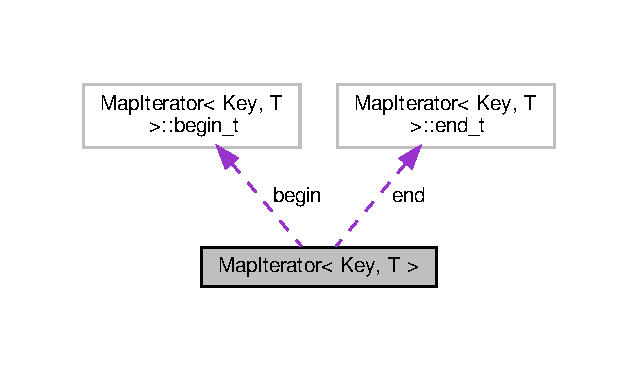
\includegraphics[width=306pt]{classMapIterator__coll__graph}
\end{center}
\end{figure}
\subsection*{Public Types}
\begin{DoxyCompactItemize}
\item 
\mbox{\Hypertarget{classMapIterator_a0e4864213515d9eac874cdfcedca6471}\label{classMapIterator_a0e4864213515d9eac874cdfcedca6471}} 
typedef \hyperlink{classMap}{Map}$<$ Key, T $>$ {\bfseries container\+\_\+type}
\item 
\mbox{\Hypertarget{classMapIterator_af7fd1f23ad34734d4a40a1ff0175c2b8}\label{classMapIterator_af7fd1f23ad34734d4a40a1ff0175c2b8}} 
typedef std\+::input\+\_\+iterator\+\_\+tag {\bfseries iterator\+\_\+category}
\item 
\mbox{\Hypertarget{classMapIterator_a64f514ba6181c3210b2712848d1e4659}\label{classMapIterator_a64f514ba6181c3210b2712848d1e4659}} 
typedef ptrdiff\+\_\+t {\bfseries difference\+\_\+type}
\item 
\mbox{\Hypertarget{classMapIterator_af9d26e048bb4713c0d748d06c000a84d}\label{classMapIterator_af9d26e048bb4713c0d748d06c000a84d}} 
typedef T $\ast$ {\bfseries pointer}
\item 
\mbox{\Hypertarget{classMapIterator_a45e98fa2e2cccd8f228a8367d5615f51}\label{classMapIterator_a45e98fa2e2cccd8f228a8367d5615f51}} 
typedef T \& {\bfseries reference}
\item 
\mbox{\Hypertarget{classMapIterator_a14cdbf4a06035dee846e299ba371b6b2}\label{classMapIterator_a14cdbf4a06035dee846e299ba371b6b2}} 
typedef container\+\_\+type\+::mapped\+\_\+type {\bfseries mapped\+\_\+type}
\item 
\mbox{\Hypertarget{classMapIterator_a1994b9d365b07113c9ab428dd8d99d08}\label{classMapIterator_a1994b9d365b07113c9ab428dd8d99d08}} 
typedef \hyperlink{classMap_a430e42d1c6a02e95eb3a34626e313441}{container\+\_\+type\+::key\+\_\+type} {\bfseries key\+\_\+type}
\item 
\mbox{\Hypertarget{classMapIterator_aa8c36b9be77994e93a7988f1f0c4edf8}\label{classMapIterator_aa8c36b9be77994e93a7988f1f0c4edf8}} 
typedef container\+\_\+type\+::value\+\_\+type {\bfseries value\+\_\+type}
\end{DoxyCompactItemize}
\subsection*{Public Member Functions}
\begin{DoxyCompactItemize}
\item 
\mbox{\Hypertarget{classMapIterator_a4a597df0199f1efc959b087be5a3c0a1}\label{classMapIterator_a4a597df0199f1efc959b087be5a3c0a1}} 
{\bfseries Map\+Iterator} (\hyperlink{classMap}{container\+\_\+type} \&map, \hyperlink{structrb__iter}{rb\+\_\+iter} $\ast$ptr)
\item 
\mbox{\Hypertarget{classMapIterator_a43fcc4ceaf1341a460fe10f0f8c1970e}\label{classMapIterator_a43fcc4ceaf1341a460fe10f0f8c1970e}} 
{\bfseries Map\+Iterator} (\hyperlink{classMap}{container\+\_\+type} \&map, const decltype(begin)\&)
\item 
\mbox{\Hypertarget{classMapIterator_a6d34d33e264c28ea94b63bc0fcb2d630}\label{classMapIterator_a6d34d33e264c28ea94b63bc0fcb2d630}} 
{\bfseries Map\+Iterator} (\hyperlink{classMap}{container\+\_\+type} \&map, const decltype(end)\&)
\item 
\mbox{\Hypertarget{classMapIterator_a5861ef9d22090c35f7c3a0287c701afd}\label{classMapIterator_a5861ef9d22090c35f7c3a0287c701afd}} 
{\bfseries Map\+Iterator} (const \hyperlink{classMapIterator}{Map\+Iterator} \&copy)
\item 
\mbox{\Hypertarget{classMapIterator_a5315a6bb774cd431a6dbe41be56828e6}\label{classMapIterator_a5315a6bb774cd431a6dbe41be56828e6}} 
\hyperlink{classMapIterator}{Map\+Iterator} \& {\bfseries operator=} (const \hyperlink{classMapIterator}{Map\+Iterator} \&copy)
\item 
\mbox{\Hypertarget{classMapIterator_adf98d3f682253cb4b8e64a1cdc24d7d1}\label{classMapIterator_adf98d3f682253cb4b8e64a1cdc24d7d1}} 
bool {\bfseries operator!=} (const \hyperlink{classMapIterator}{Map\+Iterator} \&other) const
\item 
\mbox{\Hypertarget{classMapIterator_a1c266e0517a5791e791b327d40f5ce99}\label{classMapIterator_a1c266e0517a5791e791b327d40f5ce99}} 
bool {\bfseries operator==} (const \hyperlink{classMapIterator}{Map\+Iterator} \&other) const
\item 
\mbox{\Hypertarget{classMapIterator_a5d56804c2f1d6132b5668a4e5ee699c5}\label{classMapIterator_a5d56804c2f1d6132b5668a4e5ee699c5}} 
\hyperlink{classMapIterator}{Map\+Iterator} \& {\bfseries operator++} ()
\item 
\mbox{\Hypertarget{classMapIterator_a3584d6f39ef2b74ceda095cb18e9e614}\label{classMapIterator_a3584d6f39ef2b74ceda095cb18e9e614}} 
\hyperlink{classMapIterator}{Map\+Iterator} \& {\bfseries operator-\/-\/} ()
\item 
\mbox{\Hypertarget{classMapIterator_a5325635088a46c712a6e91026a252906}\label{classMapIterator_a5325635088a46c712a6e91026a252906}} 
value\+\_\+type \& {\bfseries operator$\ast$} ()
\item 
\mbox{\Hypertarget{classMapIterator_a6ad9a230f77f15bfd6ade75e5b95bfb0}\label{classMapIterator_a6ad9a230f77f15bfd6ade75e5b95bfb0}} 
value\+\_\+type $\ast$ {\bfseries operator-\/$>$} ()
\end{DoxyCompactItemize}
\subsection*{Static Public Attributes}
\begin{DoxyCompactItemize}
\item 
\mbox{\Hypertarget{classMapIterator_a4ce43a10c73bb98307d40f6afcbf101c}\label{classMapIterator_a4ce43a10c73bb98307d40f6afcbf101c}} 
static constexpr begin\+\_\+t {\bfseries begin} = \{\}
\item 
\mbox{\Hypertarget{classMapIterator_a00c4e49846b05c748ed93575610c79b0}\label{classMapIterator_a00c4e49846b05c748ed93575610c79b0}} 
static constexpr end\+\_\+t {\bfseries end} = \{\}
\end{DoxyCompactItemize}


\subsection{Detailed Description}
\subsubsection*{template$<$typename Key, typename T$>$\newline
class Map\+Iterator$<$ Key, T $>$}

Class \hyperlink{classMapIterator}{Map\+Iterator} 

The documentation for this class was generated from the following file\+:\begin{DoxyCompactItemize}
\item 
src/map/Map.\+h\end{DoxyCompactItemize}

\hypertarget{classMultimap}{}\section{Multimap$<$ Key, T, Compare $>$ Class Template Reference}
\label{classMultimap}\index{Multimap$<$ Key, T, Compare $>$@{Multimap$<$ Key, T, Compare $>$}}


{\ttfamily \#include $<$Multimap.\+h$>$}

\subsection*{Classes}
\begin{DoxyCompactItemize}
\item 
class \hyperlink{classMultimap_1_1value__compare}{value\+\_\+compare}
\begin{DoxyCompactList}\small\item\em Classe qui compare les paires. \end{DoxyCompactList}\end{DoxyCompactItemize}
\subsection*{Public Types}
\begin{DoxyCompactItemize}
\item 
\mbox{\Hypertarget{classMultimap_ae22db357048c65265607ed263469918d}\label{classMultimap_ae22db357048c65265607ed263469918d}} 
typedef Key {\bfseries key\+\_\+type}
\item 
\mbox{\Hypertarget{classMultimap_a05f3a4a83bf4fc44da7d88ea3ef49ed5}\label{classMultimap_a05f3a4a83bf4fc44da7d88ea3ef49ed5}} 
typedef T {\bfseries mapped\+\_\+type}
\item 
\mbox{\Hypertarget{classMultimap_a0ed55c312df37a00f0e73e9c1e8b6c5a}\label{classMultimap_a0ed55c312df37a00f0e73e9c1e8b6c5a}} 
typedef std\+::pair$<$ const Key, T $>$ {\bfseries value\+\_\+type}
\item 
\mbox{\Hypertarget{classMultimap_a0e34e37c96a3fac89b7f4356e009b68e}\label{classMultimap_a0e34e37c96a3fac89b7f4356e009b68e}} 
typedef std\+::size\+\_\+t {\bfseries size\+\_\+type}
\item 
\mbox{\Hypertarget{classMultimap_a26a14e64d590f53dc692a140e99c5def}\label{classMultimap_a26a14e64d590f53dc692a140e99c5def}} 
typedef std\+::ptrdiff\+\_\+t {\bfseries difference\+\_\+type}
\item 
\mbox{\Hypertarget{classMultimap_a0c878dfdc488ba3bc9bff27e4ef74f17}\label{classMultimap_a0c878dfdc488ba3bc9bff27e4ef74f17}} 
typedef Compare {\bfseries key\+\_\+compare}
\item 
\mbox{\Hypertarget{classMultimap_a2896c71d81bb4299b7caba9df18ac617}\label{classMultimap_a2896c71d81bb4299b7caba9df18ac617}} 
typedef std\+::allocator$<$ value\+\_\+type $>$ {\bfseries allocator\+\_\+type}
\item 
\mbox{\Hypertarget{classMultimap_a1d37960f96bedba53634646633eb7943}\label{classMultimap_a1d37960f96bedba53634646633eb7943}} 
typedef T \& {\bfseries reference}
\item 
\mbox{\Hypertarget{classMultimap_a315588177f9e7a0298b43c2accbdc090}\label{classMultimap_a315588177f9e7a0298b43c2accbdc090}} 
typedef const T \& {\bfseries const\+\_\+reference}
\item 
\mbox{\Hypertarget{classMultimap_ae3dae15312101b0b6e43e5830261d297}\label{classMultimap_ae3dae15312101b0b6e43e5830261d297}} 
typedef T $\ast$ {\bfseries pointer}
\item 
\mbox{\Hypertarget{classMultimap_a9a04e5deacadfdab82e96fb85fcc2624}\label{classMultimap_a9a04e5deacadfdab82e96fb85fcc2624}} 
typedef const T $\ast$ {\bfseries const\+\_\+pointer}
\item 
\mbox{\Hypertarget{classMultimap_a1411bc48d807b5d76f464c2b3b336cd5}\label{classMultimap_a1411bc48d807b5d76f464c2b3b336cd5}} 
typedef \hyperlink{classMultimapIterator}{Multimap\+Iterator}$<$ Key, T, Compare, false $>$ {\bfseries iterator}
\item 
\mbox{\Hypertarget{classMultimap_a66040479cb2f5724f3ee62565c95d099}\label{classMultimap_a66040479cb2f5724f3ee62565c95d099}} 
typedef \hyperlink{classMultimapIterator}{Multimap\+Iterator}$<$ Key, T, Compare, true $>$ {\bfseries const\+\_\+iterator}
\end{DoxyCompactItemize}
\subsection*{Public Member Functions}
\begin{DoxyCompactItemize}
\item 
\mbox{\Hypertarget{classMultimap_acf143964f64ab59e58833b0e677f709e}\label{classMultimap_acf143964f64ab59e58833b0e677f709e}} 
\hyperlink{classMultimap_acf143964f64ab59e58833b0e677f709e}{Multimap} ()
\begin{DoxyCompactList}\small\item\em Constructeur par défaut, testé dans Test\+Constructor.\+cpp. \end{DoxyCompactList}\item 
\mbox{\Hypertarget{classMultimap_ad56590d8375c5b731bf6844d0d16822d}\label{classMultimap_ad56590d8375c5b731bf6844d0d16822d}} 
\hyperlink{classMultimap_ad56590d8375c5b731bf6844d0d16822d}{Multimap} (const Compare \&comp)
\begin{DoxyCompactList}\small\item\em Constructeur par comparateur, testé dans Test\+Constructor.\+cpp. \end{DoxyCompactList}\item 
\mbox{\Hypertarget{classMultimap_a9dd081d1a48c837b33e267e2e96aa816}\label{classMultimap_a9dd081d1a48c837b33e267e2e96aa816}} 
{\footnotesize template$<$typename Input\+It $>$ }\\\hyperlink{classMultimap_a9dd081d1a48c837b33e267e2e96aa816}{Multimap} (Input\+It first, Input\+It last, const Compare \&comp=Compare())
\begin{DoxyCompactList}\small\item\em Constructeur par intervalle d\textquotesingle{}itérateurs, testé dans Test\+Constructor.\+cpp. \end{DoxyCompactList}\item 
\mbox{\Hypertarget{classMultimap_a905d5cd2b3538dd923ff5102a75f6aab}\label{classMultimap_a905d5cd2b3538dd923ff5102a75f6aab}} 
\hyperlink{classMultimap_a905d5cd2b3538dd923ff5102a75f6aab}{Multimap} (const \hyperlink{classMultimap}{Multimap} \&other)
\begin{DoxyCompactList}\small\item\em Constructeur par copie, testé dans Test\+Constructor.\+cpp. \end{DoxyCompactList}\item 
\mbox{\Hypertarget{classMultimap_aa3f51fa1d077ccbfa1c748ebf80157c2}\label{classMultimap_aa3f51fa1d077ccbfa1c748ebf80157c2}} 
\hyperlink{classMultimap_aa3f51fa1d077ccbfa1c748ebf80157c2}{Multimap} (\hyperlink{classMultimap}{Multimap} \&\&other)
\begin{DoxyCompactList}\small\item\em Constructeur par déplacement, testé dans Test\+Constructor.\+cpp. \end{DoxyCompactList}\item 
\mbox{\Hypertarget{classMultimap_a2bb5eb1ee2f11f05f951d6b0677ea3d7}\label{classMultimap_a2bb5eb1ee2f11f05f951d6b0677ea3d7}} 
\hyperlink{classMultimap_a2bb5eb1ee2f11f05f951d6b0677ea3d7}{Multimap} (std\+::initializer\+\_\+list$<$ value\+\_\+type $>$ init, const Compare \&comp=Compare())
\begin{DoxyCompactList}\small\item\em Constructeur par liste d\textquotesingle{}initialisation, testé dans Test\+Constructor.\+cpp. \end{DoxyCompactList}\item 
\mbox{\Hypertarget{classMultimap_a99e84047761c033582cc928287fdb3be}\label{classMultimap_a99e84047761c033582cc928287fdb3be}} 
\hyperlink{classMultimap_a99e84047761c033582cc928287fdb3be}{Multimap} (const stl\+\_\+type \&other)
\begin{DoxyCompactList}\small\item\em Constructeur par copie de std\+::multimap. \end{DoxyCompactList}\item 
\mbox{\Hypertarget{classMultimap_af0f32de8dd8717d521570941dbaf2edb}\label{classMultimap_af0f32de8dd8717d521570941dbaf2edb}} 
\hyperlink{classMultimap_af0f32de8dd8717d521570941dbaf2edb}{Multimap} (stl\+\_\+type \&\&other)
\begin{DoxyCompactList}\small\item\em Constructeur par déplacement de std\+::multimap. \end{DoxyCompactList}\item 
\mbox{\Hypertarget{classMultimap_a3927ca00ca8f9363c3c73353c124348a}\label{classMultimap_a3927ca00ca8f9363c3c73353c124348a}} 
\hyperlink{classMultimap_a3927ca00ca8f9363c3c73353c124348a}{$\sim$\+Multimap} ()=default
\begin{DoxyCompactList}\small\item\em Destructeur. \end{DoxyCompactList}\item 
\mbox{\Hypertarget{classMultimap_a7624e69dbffb0df3e8f5010440060912}\label{classMultimap_a7624e69dbffb0df3e8f5010440060912}} 
\hyperlink{classMultimap}{Multimap} \& \hyperlink{classMultimap_a7624e69dbffb0df3e8f5010440060912}{operator=} (const \hyperlink{classMultimap}{Multimap} \&other)
\begin{DoxyCompactList}\small\item\em Constructeur par copie, testé dans Test\+Constructor.\+cpp. \end{DoxyCompactList}\item 
\mbox{\Hypertarget{classMultimap_a313be5fe73cd69bbcf2b2c029d8fbc4a}\label{classMultimap_a313be5fe73cd69bbcf2b2c029d8fbc4a}} 
\hyperlink{classMultimap}{Multimap} \& \hyperlink{classMultimap_a313be5fe73cd69bbcf2b2c029d8fbc4a}{operator=} (\hyperlink{classMultimap}{Multimap} \&\&other)
\begin{DoxyCompactList}\small\item\em Assignation par déplacement. \end{DoxyCompactList}\item 
\mbox{\Hypertarget{classMultimap_af4b74462f9b465dc21807083367f623b}\label{classMultimap_af4b74462f9b465dc21807083367f623b}} 
\hyperlink{classMultimap}{Multimap} \& \hyperlink{classMultimap_af4b74462f9b465dc21807083367f623b}{operator=} (std\+::initializer\+\_\+list$<$ value\+\_\+type $>$ list)
\begin{DoxyCompactList}\small\item\em Assignation par liste d\textquotesingle{}initialisation, testé dans Test\+Constructor.\+cpp. \end{DoxyCompactList}\item 
\mbox{\Hypertarget{classMultimap_a1f0ece045c7938df1f583eb76928b32a}\label{classMultimap_a1f0ece045c7938df1f583eb76928b32a}} 
\hyperlink{classMultimap}{Multimap} \& \hyperlink{classMultimap_a1f0ece045c7938df1f583eb76928b32a}{operator=} (const std\+::map$<$ Key, T, Compare $>$ \&other)
\begin{DoxyCompactList}\small\item\em Assignation par copie de std\+::multimap. \end{DoxyCompactList}\item 
\mbox{\Hypertarget{classMultimap_a339929d8a0ef5a1a2ec4f082e2e456b6}\label{classMultimap_a339929d8a0ef5a1a2ec4f082e2e456b6}} 
\hyperlink{classMultimap}{Multimap} \& \hyperlink{classMultimap_a339929d8a0ef5a1a2ec4f082e2e456b6}{operator=} (std\+::map$<$ Key, T, Compare $>$ \&\&other)
\begin{DoxyCompactList}\small\item\em Assignation par déplacement de std\+::multimap. \end{DoxyCompactList}\item 
\mbox{\Hypertarget{classMultimap_a9c10ccfcca7dd81119454f0f1f9e7b06}\label{classMultimap_a9c10ccfcca7dd81119454f0f1f9e7b06}} 
allocator\+\_\+type \hyperlink{classMultimap_a9c10ccfcca7dd81119454f0f1f9e7b06}{get\+\_\+allocator} () const
\begin{DoxyCompactList}\small\item\em Récupérer l\textquotesingle{}allocateur. \end{DoxyCompactList}\item 
\mbox{\Hypertarget{classMultimap_a4dd20f4e80f4a06be0c0fb693dd6f422}\label{classMultimap_a4dd20f4e80f4a06be0c0fb693dd6f422}} 
\hyperlink{classMultimapIterator}{iterator} \hyperlink{classMultimap_a4dd20f4e80f4a06be0c0fb693dd6f422}{begin} ()
\begin{DoxyCompactList}\small\item\em Testé dans Test\+Iterator.\+cpp. \end{DoxyCompactList}\item 
\mbox{\Hypertarget{classMultimap_aa5e3a708e644da57ac887e1acddec409}\label{classMultimap_aa5e3a708e644da57ac887e1acddec409}} 
\hyperlink{classMultimapIterator}{const\+\_\+iterator} \hyperlink{classMultimap_aa5e3a708e644da57ac887e1acddec409}{begin} () const
\begin{DoxyCompactList}\small\item\em Testé dans Test\+Iterator.\+cpp. \end{DoxyCompactList}\item 
\hyperlink{classMultimapIterator}{const\+\_\+iterator} \hyperlink{classMultimap_a216f03259a422977ea001d281a810248}{cbegin} () const
\item 
\mbox{\Hypertarget{classMultimap_a9951e49f57fe1c3984d78543eb2d9041}\label{classMultimap_a9951e49f57fe1c3984d78543eb2d9041}} 
\hyperlink{classMultimapIterator}{iterator} \hyperlink{classMultimap_a9951e49f57fe1c3984d78543eb2d9041}{end} ()
\begin{DoxyCompactList}\small\item\em Testé dans Test\+Iterator.\+cpp. \end{DoxyCompactList}\item 
\mbox{\Hypertarget{classMultimap_aee637556495f8eacebf27e95e4b9bbf6}\label{classMultimap_aee637556495f8eacebf27e95e4b9bbf6}} 
\hyperlink{classMultimapIterator}{const\+\_\+iterator} \hyperlink{classMultimap_aee637556495f8eacebf27e95e4b9bbf6}{end} () const
\begin{DoxyCompactList}\small\item\em Testé dans Test\+Iterator.\+cpp. \end{DoxyCompactList}\item 
\hyperlink{classMultimapIterator}{const\+\_\+iterator} \hyperlink{classMultimap_a7e162ec76d003b3f888c8859a9b6ca03}{cend} () const
\item 
\mbox{\Hypertarget{classMultimap_a50846e3c6ae86f987ab0cba0509f204e}\label{classMultimap_a50846e3c6ae86f987ab0cba0509f204e}} 
bool \hyperlink{classMultimap_a50846e3c6ae86f987ab0cba0509f204e}{empty} () const
\begin{DoxyCompactList}\small\item\em Testé dans Test\+Lookup.\+cpp. \end{DoxyCompactList}\item 
\mbox{\Hypertarget{classMultimap_a159de5dca46aeb29f074c6414af7bb3a}\label{classMultimap_a159de5dca46aeb29f074c6414af7bb3a}} 
size\+\_\+type \hyperlink{classMultimap_a159de5dca46aeb29f074c6414af7bb3a}{size} () const
\begin{DoxyCompactList}\small\item\em Testé dans diverses méthodes l\textquotesingle{}utilisant. \end{DoxyCompactList}\item 
\mbox{\Hypertarget{classMultimap_a9c0f70d780a722bee16bbb246fb62d8b}\label{classMultimap_a9c0f70d780a722bee16bbb246fb62d8b}} 
size\+\_\+type \hyperlink{classMultimap_a9c0f70d780a722bee16bbb246fb62d8b}{max\+\_\+size} () const
\begin{DoxyCompactList}\small\item\em Taille maximale théorique de l\textquotesingle{}arbre. \end{DoxyCompactList}\item 
\mbox{\Hypertarget{classMultimap_a6ca5068eecc98e16fbf0627db87e3742}\label{classMultimap_a6ca5068eecc98e16fbf0627db87e3742}} 
void \hyperlink{classMultimap_a6ca5068eecc98e16fbf0627db87e3742}{clear} ()
\begin{DoxyCompactList}\small\item\em Testé dans Test\+Modifier.\+cpp. \end{DoxyCompactList}\item 
\hyperlink{classMultimapIterator}{iterator} \hyperlink{classMultimap_a0a507d3094aaa271c3f5932c9acef378}{insert} (\hyperlink{classMultimapIterator}{iterator} position, const value\+\_\+type \&val)
\item 
\hyperlink{classMultimapIterator}{iterator} \hyperlink{classMultimap_aef5529b0f81f2262e6a9de27a5e47389}{insert} (value\+\_\+type \&\&pair)
\item 
{\footnotesize template$<$typename Input\+It $>$ }\\void \hyperlink{classMultimap_a62ba469ffdf46652eaa8ac007c590031}{insert} (Input\+It first, Input\+It last)
\item 
{\footnotesize template$<$typename U $>$ }\\\hyperlink{classMultimapIterator}{iterator} \hyperlink{classMultimap_ad4cd112230c4781aa25f66d78f858dd6}{insert} (U \&\&pair)
\item 
\mbox{\Hypertarget{classMultimap_af134f60e6bcb55a66618d45216c1eef9}\label{classMultimap_af134f60e6bcb55a66618d45216c1eef9}} 
size\+\_\+type \hyperlink{classMultimap_af134f60e6bcb55a66618d45216c1eef9}{erase} (const key\+\_\+type \&key)
\begin{DoxyCompactList}\small\item\em Testé dans Test\+Modifier.\+cpp. \end{DoxyCompactList}\item 
\mbox{\Hypertarget{classMultimap_a96fdc3f12cbd0af9188dbe556fe0022e}\label{classMultimap_a96fdc3f12cbd0af9188dbe556fe0022e}} 
void \hyperlink{classMultimap_a96fdc3f12cbd0af9188dbe556fe0022e}{erase} (\hyperlink{classMultimapIterator}{iterator} first, \hyperlink{classMultimapIterator}{iterator} last)
\begin{DoxyCompactList}\small\item\em Testé dans Test\+Modifier.\+cpp. \end{DoxyCompactList}\item 
\mbox{\Hypertarget{classMultimap_a9e9a35856b2ec08ffe2e05c9e97033e9}\label{classMultimap_a9e9a35856b2ec08ffe2e05c9e97033e9}} 
\hyperlink{classMultimapIterator}{iterator} \hyperlink{classMultimap_a9e9a35856b2ec08ffe2e05c9e97033e9}{erase} (\hyperlink{classMultimapIterator}{iterator} position)
\begin{DoxyCompactList}\small\item\em Testé dans Test\+Modifier.\+cpp. \end{DoxyCompactList}\item 
\mbox{\Hypertarget{classMultimap_aacaf7aaeab79c30b3a19b85a10a56f7c}\label{classMultimap_aacaf7aaeab79c30b3a19b85a10a56f7c}} 
void \hyperlink{classMultimap_aacaf7aaeab79c30b3a19b85a10a56f7c}{swap} (\hyperlink{classMultimap}{Multimap} \&other)
\begin{DoxyCompactList}\small\item\em Algorithme swap spécialisé pour les multimap. \end{DoxyCompactList}\item 
\mbox{\Hypertarget{classMultimap_a2feb4082ad4884bc49e68bb4815769db}\label{classMultimap_a2feb4082ad4884bc49e68bb4815769db}} 
size\+\_\+type \hyperlink{classMultimap_a2feb4082ad4884bc49e68bb4815769db}{count} (const key\+\_\+type \&key)
\begin{DoxyCompactList}\small\item\em Testé dans Test\+Lookup.\+cpp. \end{DoxyCompactList}\item 
\mbox{\Hypertarget{classMultimap_a111dfc88089590ec1f94de7e6e3d2715}\label{classMultimap_a111dfc88089590ec1f94de7e6e3d2715}} 
\hyperlink{classMultimapIterator}{iterator} \hyperlink{classMultimap_a111dfc88089590ec1f94de7e6e3d2715}{find} (const key\+\_\+type \&key)
\begin{DoxyCompactList}\small\item\em Testé dans Test\+Lookup.\+cpp. \end{DoxyCompactList}\item 
\mbox{\Hypertarget{classMultimap_a0fa9b709bbb25ef657d7ff8f70402203}\label{classMultimap_a0fa9b709bbb25ef657d7ff8f70402203}} 
bool \hyperlink{classMultimap_a0fa9b709bbb25ef657d7ff8f70402203}{contains} (const Key \&key)
\begin{DoxyCompactList}\small\item\em Testé dans Test\+Lookup.\+cpp (C++20) \end{DoxyCompactList}\item 
\mbox{\Hypertarget{classMultimap_a7402d5ca0eead6166d93e8fa154bdeee}\label{classMultimap_a7402d5ca0eead6166d93e8fa154bdeee}} 
std\+::pair$<$ \hyperlink{classMultimapIterator}{iterator}, \hyperlink{classMultimapIterator}{iterator} $>$ {\bfseries equal\+\_\+range} (const Key \&key)
\item 
\mbox{\Hypertarget{classMultimap_a987440eb1d580fc0d8231857e27517b4}\label{classMultimap_a987440eb1d580fc0d8231857e27517b4}} 
\hyperlink{classMultimapIterator}{iterator} \hyperlink{classMultimap_a987440eb1d580fc0d8231857e27517b4}{lower\+\_\+bound} (const key\+\_\+type \&key)
\begin{DoxyCompactList}\small\item\em Testé dans Test\+Lookup.\+cpp. \end{DoxyCompactList}\item 
\mbox{\Hypertarget{classMultimap_a5cef442af3427edbe14da2668e2c59cd}\label{classMultimap_a5cef442af3427edbe14da2668e2c59cd}} 
\hyperlink{classMultimapIterator}{iterator} \hyperlink{classMultimap_a5cef442af3427edbe14da2668e2c59cd}{upper\+\_\+bound} (const key\+\_\+type \&key)
\begin{DoxyCompactList}\small\item\em Testé dans Test\+Lookup.\+cpp (C++20) \end{DoxyCompactList}\item 
\mbox{\Hypertarget{classMultimap_ae49e443fd752bd5954b50f1b8fbaa5c4}\label{classMultimap_ae49e443fd752bd5954b50f1b8fbaa5c4}} 
key\+\_\+compare {\bfseries key\+\_\+comp} () const
\item 
\mbox{\Hypertarget{classMultimap_a4d832c78ba715b043a078e56dc376aea}\label{classMultimap_a4d832c78ba715b043a078e56dc376aea}} 
\hyperlink{classMultimap_1_1value__compare}{value\+\_\+compare} {\bfseries value\+\_\+comp} () const
\item 
\mbox{\Hypertarget{classMultimap_ad912308e6c19b562697ab713b0ccdd33}\label{classMultimap_ad912308e6c19b562697ab713b0ccdd33}} 
bool {\bfseries equals} (const std\+::initializer\+\_\+list$<$ value\+\_\+type $>$ \&il) const
\item 
\mbox{\Hypertarget{classMultimap_a90017019b311b34d667a7b0962fe1d13}\label{classMultimap_a90017019b311b34d667a7b0962fe1d13}} 
{\footnotesize template$<$typename Input\+It $>$ }\\bool \hyperlink{classMultimap_a90017019b311b34d667a7b0962fe1d13}{equals} (Input\+It first, Input\+It last) const
\begin{DoxyCompactList}\small\item\em Comparaison à un intervalle d\textquotesingle{}itérateurs Retourne vrai si les contenus sont strictement indentiques. \end{DoxyCompactList}\end{DoxyCompactItemize}
\subsection*{Public Attributes}
\begin{DoxyCompactItemize}
\item 
\mbox{\Hypertarget{classMultimap_a2f1ded72848f333473e2e5d74f510474}\label{classMultimap_a2f1ded72848f333473e2e5d74f510474}} 
friend \hyperlink{classMultimap_a2f1ded72848f333473e2e5d74f510474}{Multimap\+Iterator$<$ Key, T, Compare, false $>$}
\begin{DoxyCompactList}\small\item\em Itérateur non constant. \end{DoxyCompactList}\item 
\mbox{\Hypertarget{classMultimap_afbda4125c5317ddde9caff060b3d82d6}\label{classMultimap_afbda4125c5317ddde9caff060b3d82d6}} 
friend \hyperlink{classMultimap_afbda4125c5317ddde9caff060b3d82d6}{Multimap\+Iterator$<$ Key, T, Compare, true $>$}
\begin{DoxyCompactList}\small\item\em Itérateur constant. \end{DoxyCompactList}\end{DoxyCompactItemize}
\subsection*{Friends}
\begin{DoxyCompactItemize}
\item 
\mbox{\Hypertarget{classMultimap_a6a1747a11110a47ddccb947d8727c1db}\label{classMultimap_a6a1747a11110a47ddccb947d8727c1db}} 
bool {\bfseries operator==} (const \hyperlink{classMultimap}{Multimap} \&lhs, const \hyperlink{classMultimap}{Multimap} \&rhs)
\item 
\mbox{\Hypertarget{classMultimap_aa727e58dd28602ada5511260bc380d92}\label{classMultimap_aa727e58dd28602ada5511260bc380d92}} 
bool {\bfseries operator==} (const \hyperlink{classMultimap}{Multimap} \&lhs, const stl\+\_\+type \&rhs)
\item 
\mbox{\Hypertarget{classMultimap_aca3fa84add2579de08ecae95debb4d4d}\label{classMultimap_aca3fa84add2579de08ecae95debb4d4d}} 
bool {\bfseries operator==} (const stl\+\_\+type \&lhs, const \hyperlink{classMultimap}{Multimap} \&rhs)
\item 
\mbox{\Hypertarget{classMultimap_aa11fe172d670ef1bbb20888e437bed4b}\label{classMultimap_aa11fe172d670ef1bbb20888e437bed4b}} 
bool {\bfseries operator!=} (const \hyperlink{classMultimap}{Multimap} \&lhs, const \hyperlink{classMultimap}{Multimap} \&rhs)
\item 
\mbox{\Hypertarget{classMultimap_ae4bcd97f54c81f8947d18451137c1bfe}\label{classMultimap_ae4bcd97f54c81f8947d18451137c1bfe}} 
bool {\bfseries operator!=} (const \hyperlink{classMultimap}{Multimap} \&lhs, const stl\+\_\+type \&rhs)
\item 
\mbox{\Hypertarget{classMultimap_a977585e743d4f074d345ed129b0e0853}\label{classMultimap_a977585e743d4f074d345ed129b0e0853}} 
bool {\bfseries operator!=} (const stl\+\_\+type \&lhs, const \hyperlink{classMultimap}{Multimap} \&rhs)
\item 
std\+::ostream \& \hyperlink{classMultimap_a3a9cc0a79670c0bf02221d1cde83e1e0}{operator$<$$<$} (std\+::ostream \&lhs, const \hyperlink{classMultimap}{Multimap} \&rhs)
\end{DoxyCompactItemize}


\subsection{Detailed Description}
\subsubsection*{template$<$class Key, class T, class Compare$>$\newline
class Multimap$<$ Key, T, Compare $>$}

Ordre des déclarations (alias/prototypes) Selon \href{https://en.cppreference.com/w/cpp/container/multimap}{\tt https\+://en.\+cppreference.\+com/w/cpp/container/multimap} Trié par surcharge, dans l\textquotesingle{}ordre aussi, mis à part structure interne 

\subsection{Member Function Documentation}
\mbox{\Hypertarget{classMultimap_a216f03259a422977ea001d281a810248}\label{classMultimap_a216f03259a422977ea001d281a810248}} 
\index{Multimap@{Multimap}!cbegin@{cbegin}}
\index{cbegin@{cbegin}!Multimap@{Multimap}}
\subsubsection{\texorpdfstring{cbegin()}{cbegin()}}
{\footnotesize\ttfamily template$<$class Key , class T , class Compare $>$ \\
\hyperlink{classMultimapIterator}{const\+\_\+iterator} \hyperlink{classMultimap}{Multimap}$<$ Key, T, Compare $>$\+::cbegin (\begin{DoxyParamCaption}{ }\end{DoxyParamCaption}) const\hspace{0.3cm}{\ttfamily [inline]}}

Itérateur de début constant Testé dans Test\+Iterator.\+cpp \mbox{\Hypertarget{classMultimap_a7e162ec76d003b3f888c8859a9b6ca03}\label{classMultimap_a7e162ec76d003b3f888c8859a9b6ca03}} 
\index{Multimap@{Multimap}!cend@{cend}}
\index{cend@{cend}!Multimap@{Multimap}}
\subsubsection{\texorpdfstring{cend()}{cend()}}
{\footnotesize\ttfamily template$<$class Key , class T , class Compare $>$ \\
\hyperlink{classMultimapIterator}{const\+\_\+iterator} \hyperlink{classMultimap}{Multimap}$<$ Key, T, Compare $>$\+::cend (\begin{DoxyParamCaption}{ }\end{DoxyParamCaption}) const\hspace{0.3cm}{\ttfamily [inline]}}

Itérateur de past-\/the-\/end constant Testé dans Test\+Iterator.\+cpp \mbox{\Hypertarget{classMultimap_a0a507d3094aaa271c3f5932c9acef378}\label{classMultimap_a0a507d3094aaa271c3f5932c9acef378}} 
\index{Multimap@{Multimap}!insert@{insert}}
\index{insert@{insert}!Multimap@{Multimap}}
\subsubsection{\texorpdfstring{insert()}{insert()}\hspace{0.1cm}{\footnotesize\ttfamily [1/4]}}
{\footnotesize\ttfamily template$<$class Key , class T , class Compare $>$ \\
\hyperlink{classMultimapIterator}{iterator} \hyperlink{classMultimap}{Multimap}$<$ Key, T, Compare $>$\+::insert (\begin{DoxyParamCaption}\item[{\hyperlink{classMultimapIterator}{iterator}}]{position,  }\item[{const value\+\_\+type \&}]{val }\end{DoxyParamCaption})\hspace{0.3cm}{\ttfamily [inline]}}

Insertion en conaissant déjà la position de l\textquotesingle{}élément Testé dans Test\+Modifier.\+cpp \mbox{\Hypertarget{classMultimap_aef5529b0f81f2262e6a9de27a5e47389}\label{classMultimap_aef5529b0f81f2262e6a9de27a5e47389}} 
\index{Multimap@{Multimap}!insert@{insert}}
\index{insert@{insert}!Multimap@{Multimap}}
\subsubsection{\texorpdfstring{insert()}{insert()}\hspace{0.1cm}{\footnotesize\ttfamily [2/4]}}
{\footnotesize\ttfamily template$<$class Key , class T , class Compare $>$ \\
\hyperlink{classMultimapIterator}{iterator} \hyperlink{classMultimap}{Multimap}$<$ Key, T, Compare $>$\+::insert (\begin{DoxyParamCaption}\item[{value\+\_\+type \&\&}]{pair }\end{DoxyParamCaption})\hspace{0.3cm}{\ttfamily [inline]}}

Surcharge par rapport à la fonction template pour permettre l\textquotesingle{}appel par liste d\textquotesingle{}initialisation Testé dans Test\+Modifier.\+cpp \mbox{\Hypertarget{classMultimap_a62ba469ffdf46652eaa8ac007c590031}\label{classMultimap_a62ba469ffdf46652eaa8ac007c590031}} 
\index{Multimap@{Multimap}!insert@{insert}}
\index{insert@{insert}!Multimap@{Multimap}}
\subsubsection{\texorpdfstring{insert()}{insert()}\hspace{0.1cm}{\footnotesize\ttfamily [3/4]}}
{\footnotesize\ttfamily template$<$class Key , class T , class Compare $>$ \\
template$<$typename Input\+It $>$ \\
void \hyperlink{classMultimap}{Multimap}$<$ Key, T, Compare $>$\+::insert (\begin{DoxyParamCaption}\item[{Input\+It}]{first,  }\item[{Input\+It}]{last }\end{DoxyParamCaption})\hspace{0.3cm}{\ttfamily [inline]}}

Insertion par intervaleur d\textquotesingle{}itérateurs Testé dans Test\+Modifier.\+cpp \mbox{\Hypertarget{classMultimap_ad4cd112230c4781aa25f66d78f858dd6}\label{classMultimap_ad4cd112230c4781aa25f66d78f858dd6}} 
\index{Multimap@{Multimap}!insert@{insert}}
\index{insert@{insert}!Multimap@{Multimap}}
\subsubsection{\texorpdfstring{insert()}{insert()}\hspace{0.1cm}{\footnotesize\ttfamily [4/4]}}
{\footnotesize\ttfamily template$<$class Key , class T , class Compare $>$ \\
template$<$typename U $>$ \\
\hyperlink{classMultimapIterator}{iterator} \hyperlink{classMultimap}{Multimap}$<$ Key, T, Compare $>$\+::insert (\begin{DoxyParamCaption}\item[{U \&\&}]{pair }\end{DoxyParamCaption})\hspace{0.3cm}{\ttfamily [inline]}}


\begin{DoxyParams}{Parameters}
{\em pair} & Référence universelle Testé dans Test\+Modifier.\+cpp \\
\hline
\end{DoxyParams}


\subsection{Friends And Related Function Documentation}
\mbox{\Hypertarget{classMultimap_a3a9cc0a79670c0bf02221d1cde83e1e0}\label{classMultimap_a3a9cc0a79670c0bf02221d1cde83e1e0}} 
\index{Multimap@{Multimap}!operator$<$$<$@{operator$<$$<$}}
\index{operator$<$$<$@{operator$<$$<$}!Multimap@{Multimap}}
\subsubsection{\texorpdfstring{operator$<$$<$}{operator<<}}
{\footnotesize\ttfamily template$<$class Key , class T , class Compare $>$ \\
std\+::ostream\& operator$<$$<$ (\begin{DoxyParamCaption}\item[{std\+::ostream \&}]{lhs,  }\item[{const \hyperlink{classMultimap}{Multimap}$<$ Key, T, Compare $>$ \&}]{rhs }\end{DoxyParamCaption})\hspace{0.3cm}{\ttfamily [friend]}}

\subsubsection*{Fonctions non membres utiles }

The documentation for this class was generated from the following file\+:\begin{DoxyCompactItemize}
\item 
src/multimap/Multimap.\+h\end{DoxyCompactItemize}

\hypertarget{classMultimapIterator}{}\section{Multimap\+Iterator$<$ Key, Value, Compare, Is\+Const $>$ Class Template Reference}
\label{classMultimapIterator}\index{Multimap\+Iterator$<$ Key, Value, Compare, Is\+Const $>$@{Multimap\+Iterator$<$ Key, Value, Compare, Is\+Const $>$}}


Itérateur.  




{\ttfamily \#include $<$Multimap\+Iterator.\+h$>$}

\subsection*{Public Types}
\begin{DoxyCompactItemize}
\item 
\mbox{\Hypertarget{classMultimapIterator_a899266d0ec292bcb0cc369e5ee421434}\label{classMultimapIterator_a899266d0ec292bcb0cc369e5ee421434}} 
using {\bfseries difference\+\_\+type} = std\+::ptrdiff\+\_\+t
\item 
\mbox{\Hypertarget{classMultimapIterator_a3cdb3b8fcf5c7148a895559ed69f353f}\label{classMultimapIterator_a3cdb3b8fcf5c7148a895559ed69f353f}} 
using {\bfseries iterator\+\_\+category} = std\+::bidirectional\+\_\+iterator\+\_\+tag
\item 
\mbox{\Hypertarget{classMultimapIterator_a9c0233078690a6541aea151e6df0b3d7}\label{classMultimapIterator_a9c0233078690a6541aea151e6df0b3d7}} 
using {\bfseries value\+\_\+type} = Pair
\item 
\mbox{\Hypertarget{classMultimapIterator_aaafa1d93e40c7a18504a95661938515f}\label{classMultimapIterator_aaafa1d93e40c7a18504a95661938515f}} 
using {\bfseries pointer} = Pair $\ast$
\item 
\mbox{\Hypertarget{classMultimapIterator_a4c5da38f2cdfa8a27f7db2da46cfa2fa}\label{classMultimapIterator_a4c5da38f2cdfa8a27f7db2da46cfa2fa}} 
using {\bfseries reference} = Pair \&
\end{DoxyCompactItemize}
\subsection*{Public Member Functions}
\begin{DoxyCompactItemize}
\item 
\hyperlink{classMultimapIterator_ac8fed38e75dedfa911756c5d619e9b4a}{Multimap\+Iterator} ()
\begin{DoxyCompactList}\small\item\em Constructeurs -\/-\/-\/-\/-\/-\/-\/-\/-\/-\/------. \end{DoxyCompactList}\item 
\mbox{\Hypertarget{classMultimapIterator_a52231305c8f71648ce98993273899874}\label{classMultimapIterator_a52231305c8f71648ce98993273899874}} 
\hyperlink{classMultimapIterator_a52231305c8f71648ce98993273899874}{Multimap\+Iterator} (Container \&m)
\begin{DoxyCompactList}\small\item\em Itérateur de fin. \end{DoxyCompactList}\item 
\mbox{\Hypertarget{classMultimapIterator_a03504a7b1b57e6e5216b63561510d6fe}\label{classMultimapIterator_a03504a7b1b57e6e5216b63561510d6fe}} 
{\bfseries Multimap\+Iterator} (Container \&m, Node \&node, Single\+Node \&s)
\item 
\mbox{\Hypertarget{classMultimapIterator_a79df350144602525d2ecd5701a69c5be}\label{classMultimapIterator_a79df350144602525d2ecd5701a69c5be}} 
{\bfseries Multimap\+Iterator} (Container \&m, Node \&node, Position pos=F\+R\+O\+NT)
\item 
\mbox{\Hypertarget{classMultimapIterator_addb81cae98d05bb35e628eaa0bccb539}\label{classMultimapIterator_addb81cae98d05bb35e628eaa0bccb539}} 
\hyperlink{classMultimapIterator_addb81cae98d05bb35e628eaa0bccb539}{Multimap\+Iterator} (const \hyperlink{classMultimapIterator}{Multimap\+Iterator} \&o)
\begin{DoxyCompactList}\small\item\em Constructeur par copie. \end{DoxyCompactList}\item 
{\footnotesize template$<$bool Is\+Const\+It$>$ }\\\hyperlink{classMultimapIterator_a97311a11001e54f21fd81c22f310eb3c}{Multimap\+Iterator} (const \hyperlink{classMultimapIterator}{Multimap\+Iterator}$<$ Key, Value, Compare, Is\+Const\+It $>$ \&o)
\item 
const Key \& \hyperlink{classMultimapIterator_a016fca3267d16d48b57964ee39d9efae}{key} () const
\begin{DoxyCompactList}\small\item\em Accesseurs -\/-\/-\/-\/-\/-\/-\/-\/-\/-\/-\/-\/-\/-\/-\/------. \end{DoxyCompactList}\item 
\mbox{\Hypertarget{classMultimapIterator_a564b7e18dcbb0f5c27b0b0a7a4e38f8b}\label{classMultimapIterator_a564b7e18dcbb0f5c27b0b0a7a4e38f8b}} 
value\+\_\+type \& \hyperlink{classMultimapIterator_a564b7e18dcbb0f5c27b0b0a7a4e38f8b}{operator$\ast$} () const
\begin{DoxyCompactList}\small\item\em Récupère la paire \{clé, valeur\}. \end{DoxyCompactList}\item 
\mbox{\Hypertarget{classMultimapIterator_a1f71fdba1777563641dd148031e069d0}\label{classMultimapIterator_a1f71fdba1777563641dd148031e069d0}} 
value\+\_\+type $\ast$ {\bfseries operator-\/$>$} () const
\item 
\mbox{\Hypertarget{classMultimapIterator_a54ebc650ff944f37210e7755e2cdf9fa}\label{classMultimapIterator_a54ebc650ff944f37210e7755e2cdf9fa}} 
\hyperlink{classMultimapIterator}{Multimap\+Iterator} \& \hyperlink{classMultimapIterator_a54ebc650ff944f37210e7755e2cdf9fa}{operator++} ()
\begin{DoxyCompactList}\small\item\em Prochain élément (préfixe) \end{DoxyCompactList}\item 
\mbox{\Hypertarget{classMultimapIterator_ae012d5b9a2df03f80da41b665752a9a8}\label{classMultimapIterator_ae012d5b9a2df03f80da41b665752a9a8}} 
\hyperlink{classMultimapIterator}{Multimap\+Iterator} \hyperlink{classMultimapIterator_ae012d5b9a2df03f80da41b665752a9a8}{operator++} (int)
\begin{DoxyCompactList}\small\item\em Prochain élément (postfixe) \end{DoxyCompactList}\item 
\hyperlink{classMultimapIterator}{Multimap\+Iterator} \& \hyperlink{classMultimapIterator_a70a34f78b77e58c3137066f3515628fd}{operator-\/-\/} ()
\item 
\hyperlink{classMultimapIterator}{Multimap\+Iterator} \hyperlink{classMultimapIterator_acda65b98718a6dea2194f69dbdbcf5ee}{operator-\/-\/} (int)
\item 
\mbox{\Hypertarget{classMultimapIterator_af337db177c534cb9b9ffed2f43880e6a}\label{classMultimapIterator_af337db177c534cb9b9ffed2f43880e6a}} 
\hyperlink{classMultimapIterator}{Multimap\+Iterator} \& \hyperlink{classMultimapIterator_af337db177c534cb9b9ffed2f43880e6a}{operator=} (const \hyperlink{classMultimapIterator}{Multimap\+Iterator} \&o)
\begin{DoxyCompactList}\small\item\em Assignation par copie. \end{DoxyCompactList}\item 
{\footnotesize template$<$bool Is\+Const\+It$>$ }\\bool \hyperlink{classMultimapIterator_ad8ae7f78f86f880a611c9bc4939ec98b}{operator==} (const \hyperlink{classMultimapIterator}{Multimap\+Iterator}$<$ Key, Value, Compare, Is\+Const\+It $>$ \&rhs) const
\begin{DoxyCompactList}\small\item\em Opérateurs -\/-\/-\/-\/-\/-\/-\/-\/-\/-\/-\/-\/-\/-\/------. \end{DoxyCompactList}\item 
\mbox{\Hypertarget{classMultimapIterator_a22772d2fe41f4cd132c2a882372473e3}\label{classMultimapIterator_a22772d2fe41f4cd132c2a882372473e3}} 
{\footnotesize template$<$bool Is\+Const\+It$>$ }\\bool {\bfseries operator!=} (const \hyperlink{classMultimapIterator}{Multimap\+Iterator}$<$ Key, Value, Compare, Is\+Const\+It $>$ \&rhs) const
\end{DoxyCompactItemize}
\subsection*{Friends}
\begin{DoxyCompactItemize}
\item 
\mbox{\Hypertarget{classMultimapIterator_a6285b24f1f2750aac18f3ca3f8e1ff46}\label{classMultimapIterator_a6285b24f1f2750aac18f3ca3f8e1ff46}} 
class {\bfseries Multimap$<$ Key, Value, Compare $>$}
\item 
\mbox{\Hypertarget{classMultimapIterator_a55b0482e033ddf2d5827503cf697da34}\label{classMultimapIterator_a55b0482e033ddf2d5827503cf697da34}} 
class {\bfseries Multimap\+Iterator$<$ Key, Value, Compare, !\+Is\+Const $>$}
\end{DoxyCompactItemize}


\subsection{Detailed Description}
\subsubsection*{template$<$class Key, class Value, class Compare, bool Is\+Const$>$\newline
class Multimap\+Iterator$<$ Key, Value, Compare, Is\+Const $>$}

Itérateur. 

\subsection{Constructor \& Destructor Documentation}
\mbox{\Hypertarget{classMultimapIterator_ac8fed38e75dedfa911756c5d619e9b4a}\label{classMultimapIterator_ac8fed38e75dedfa911756c5d619e9b4a}} 
\index{Multimap\+Iterator@{Multimap\+Iterator}!Multimap\+Iterator@{Multimap\+Iterator}}
\index{Multimap\+Iterator@{Multimap\+Iterator}!Multimap\+Iterator@{Multimap\+Iterator}}
\subsubsection{\texorpdfstring{Multimap\+Iterator()}{MultimapIterator()}\hspace{0.1cm}{\footnotesize\ttfamily [1/2]}}
{\footnotesize\ttfamily template$<$class Key , class Value , class Compare , bool Is\+Const$>$ \\
\hyperlink{classMultimapIterator}{Multimap\+Iterator}$<$ Key, Value, Compare, Is\+Const $>$\+::\hyperlink{classMultimapIterator}{Multimap\+Iterator} (\begin{DoxyParamCaption}{ }\end{DoxyParamCaption})}



Constructeurs -\/-\/-\/-\/-\/-\/-\/-\/-\/-\/------. 

Construit un itérateur invalide dont la seule action valide est de l\textquotesingle{}assigner à un autre itérateur \mbox{\Hypertarget{classMultimapIterator_a97311a11001e54f21fd81c22f310eb3c}\label{classMultimapIterator_a97311a11001e54f21fd81c22f310eb3c}} 
\index{Multimap\+Iterator@{Multimap\+Iterator}!Multimap\+Iterator@{Multimap\+Iterator}}
\index{Multimap\+Iterator@{Multimap\+Iterator}!Multimap\+Iterator@{Multimap\+Iterator}}
\subsubsection{\texorpdfstring{Multimap\+Iterator()}{MultimapIterator()}\hspace{0.1cm}{\footnotesize\ttfamily [2/2]}}
{\footnotesize\ttfamily template$<$class Key, class Value, class Compare, bool Is\+Const$>$ \\
template$<$bool Is\+Const\+It$>$ \\
\hyperlink{classMultimapIterator}{Multimap\+Iterator}$<$ Key, Value, Compare, Is\+Const $>$\+::\hyperlink{classMultimapIterator}{Multimap\+Iterator} (\begin{DoxyParamCaption}\item[{const \hyperlink{classMultimapIterator}{Multimap\+Iterator}$<$ Key, Value, Compare, Is\+Const\+It $>$ \&}]{o }\end{DoxyParamCaption})\hspace{0.3cm}{\ttfamily [inline]}}

Permet la construction de const à partir de non-\/const Le constructeur par copie est préféré si Is\+Const = Is\+Const\+It 

\subsection{Member Function Documentation}
\mbox{\Hypertarget{classMultimapIterator_a016fca3267d16d48b57964ee39d9efae}\label{classMultimapIterator_a016fca3267d16d48b57964ee39d9efae}} 
\index{Multimap\+Iterator@{Multimap\+Iterator}!key@{key}}
\index{key@{key}!Multimap\+Iterator@{Multimap\+Iterator}}
\subsubsection{\texorpdfstring{key()}{key()}}
{\footnotesize\ttfamily template$<$class Key , class Value , class Compare , bool Is\+Const$>$ \\
const Key \& \hyperlink{classMultimapIterator}{Multimap\+Iterator}$<$ Key, Value, Compare, Is\+Const $>$\+::key (\begin{DoxyParamCaption}{ }\end{DoxyParamCaption}) const}



Accesseurs -\/-\/-\/-\/-\/-\/-\/-\/-\/-\/-\/-\/-\/-\/-\/------. 

Récupère la clé \mbox{\Hypertarget{classMultimapIterator_a70a34f78b77e58c3137066f3515628fd}\label{classMultimapIterator_a70a34f78b77e58c3137066f3515628fd}} 
\index{Multimap\+Iterator@{Multimap\+Iterator}!operator-\/-\/@{operator-\/-\/}}
\index{operator-\/-\/@{operator-\/-\/}!Multimap\+Iterator@{Multimap\+Iterator}}
\subsubsection{\texorpdfstring{operator-\/-\/()}{operator--()}\hspace{0.1cm}{\footnotesize\ttfamily [1/2]}}
{\footnotesize\ttfamily template$<$class Key , class Value , class Compare , bool Is\+Const$>$ \\
\hyperlink{classMultimapIterator}{Multimap\+Iterator}$<$ Key, Value, Compare, Is\+Const $>$ \& \hyperlink{classMultimapIterator}{Multimap\+Iterator}$<$ Key, Value, Compare, Is\+Const $>$\+::operator-\/-\/ (\begin{DoxyParamCaption}{ }\end{DoxyParamCaption})}

Element précédent (préfixe) Si le conteneur est vide, comportement indéfini Si c\textquotesingle{}est le premier élément, comportement indéfini \mbox{\Hypertarget{classMultimapIterator_acda65b98718a6dea2194f69dbdbcf5ee}\label{classMultimapIterator_acda65b98718a6dea2194f69dbdbcf5ee}} 
\index{Multimap\+Iterator@{Multimap\+Iterator}!operator-\/-\/@{operator-\/-\/}}
\index{operator-\/-\/@{operator-\/-\/}!Multimap\+Iterator@{Multimap\+Iterator}}
\subsubsection{\texorpdfstring{operator-\/-\/()}{operator--()}\hspace{0.1cm}{\footnotesize\ttfamily [2/2]}}
{\footnotesize\ttfamily template$<$class Key , class Value , class Compare , bool Is\+Const$>$ \\
\hyperlink{classMultimapIterator}{Multimap\+Iterator}$<$ Key, Value, Compare, Is\+Const $>$ \hyperlink{classMultimapIterator}{Multimap\+Iterator}$<$ Key, Value, Compare, Is\+Const $>$\+::operator-\/-\/ (\begin{DoxyParamCaption}\item[{int}]{ }\end{DoxyParamCaption})}

Elément précédent (postfixe) Si le conteneur est vide, comportement indéfini Si c\textquotesingle{}est le premier élément, comportement indéfini \mbox{\Hypertarget{classMultimapIterator_ad8ae7f78f86f880a611c9bc4939ec98b}\label{classMultimapIterator_ad8ae7f78f86f880a611c9bc4939ec98b}} 
\index{Multimap\+Iterator@{Multimap\+Iterator}!operator==@{operator==}}
\index{operator==@{operator==}!Multimap\+Iterator@{Multimap\+Iterator}}
\subsubsection{\texorpdfstring{operator==()}{operator==()}}
{\footnotesize\ttfamily template$<$class Key, class Value, class Compare, bool Is\+Const$>$ \\
template$<$bool Is\+Const\+It$>$ \\
bool \hyperlink{classMultimapIterator}{Multimap\+Iterator}$<$ Key, Value, Compare, Is\+Const $>$\+::operator== (\begin{DoxyParamCaption}\item[{const \hyperlink{classMultimapIterator}{Multimap\+Iterator}$<$ Key, Value, Compare, Is\+Const\+It $>$ \&}]{rhs }\end{DoxyParamCaption}) const\hspace{0.3cm}{\ttfamily [inline]}}



Opérateurs -\/-\/-\/-\/-\/-\/-\/-\/-\/-\/-\/-\/-\/-\/------. 

Egalité Deux itérateurs sont égaux s\textquotesingle{}ils pointent vers le même élément de la même multimap Dans le cas de l\textquotesingle{}itérateur de fin, il faut que se soit l\textquotesingle{}itérateur de fin des même conteneur 

The documentation for this class was generated from the following file\+:\begin{DoxyCompactItemize}
\item 
src/multimap/Multimap\+Iterator.\+h\end{DoxyCompactItemize}

\hypertarget{structrb__iter}{}\section{rb\+\_\+iter Struct Reference}
\label{structrb__iter}\index{rb\+\_\+iter@{rb\+\_\+iter}}


Collaboration diagram for rb\+\_\+iter\+:\nopagebreak
\begin{figure}[H]
\begin{center}
\leavevmode
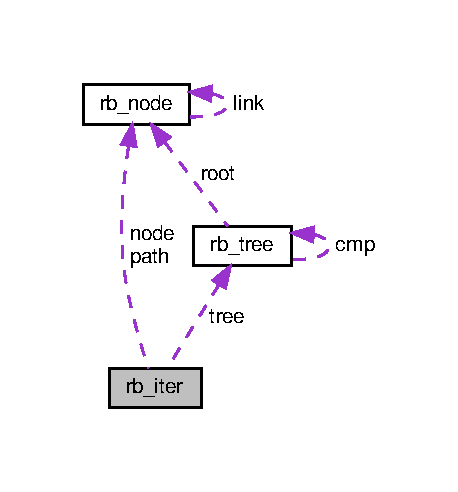
\includegraphics[width=220pt]{structrb__iter__coll__graph}
\end{center}
\end{figure}
\subsection*{Public Attributes}
\begin{DoxyCompactItemize}
\item 
\mbox{\Hypertarget{structrb__iter_aa7d16e8bd1c481afb06b660f9921c282}\label{structrb__iter_aa7d16e8bd1c481afb06b660f9921c282}} 
struct \hyperlink{structrb__tree}{rb\+\_\+tree} $\ast$ {\bfseries tree}
\item 
\mbox{\Hypertarget{structrb__iter_aa100152b6704697647b9f9c1b83b8b58}\label{structrb__iter_aa100152b6704697647b9f9c1b83b8b58}} 
struct \hyperlink{structrb__node}{rb\+\_\+node} $\ast$ {\bfseries node}
\item 
\mbox{\Hypertarget{structrb__iter_a140f9483858ea4aa231d2c242153edbc}\label{structrb__iter_a140f9483858ea4aa231d2c242153edbc}} 
struct \hyperlink{structrb__node}{rb\+\_\+node} $\ast$ {\bfseries path} \mbox{[}R\+B\+\_\+\+I\+T\+E\+R\+\_\+\+M\+A\+X\+\_\+\+H\+E\+I\+G\+HT\mbox{]}
\item 
\mbox{\Hypertarget{structrb__iter_a9f69bb4c1811ae482b9cc8962fc0eea9}\label{structrb__iter_a9f69bb4c1811ae482b9cc8962fc0eea9}} 
size\+\_\+t {\bfseries top}
\item 
\mbox{\Hypertarget{structrb__iter_a02f1339882a40f5319301767791f9b8e}\label{structrb__iter_a02f1339882a40f5319301767791f9b8e}} 
void $\ast$ {\bfseries info}
\end{DoxyCompactItemize}


The documentation for this struct was generated from the following file\+:\begin{DoxyCompactItemize}
\item 
src/map/rb\+\_\+tree.\+h\end{DoxyCompactItemize}

\hypertarget{structrb__node}{}\section{rb\+\_\+node Struct Reference}
\label{structrb__node}\index{rb\+\_\+node@{rb\+\_\+node}}


Collaboration diagram for rb\+\_\+node\+:\nopagebreak
\begin{figure}[H]
\begin{center}
\leavevmode
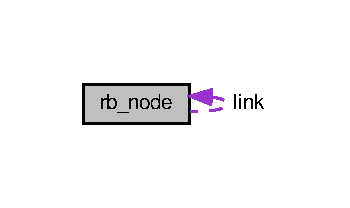
\includegraphics[width=168pt]{structrb__node__coll__graph}
\end{center}
\end{figure}
\subsection*{Public Attributes}
\begin{DoxyCompactItemize}
\item 
\mbox{\Hypertarget{structrb__node_ac12d2b253512f2ee39a14fee8e07c427}\label{structrb__node_ac12d2b253512f2ee39a14fee8e07c427}} 
int {\bfseries red}
\item 
\mbox{\Hypertarget{structrb__node_a3bd2cfafe2513fc8d59e6ea4d4f9c056}\label{structrb__node_a3bd2cfafe2513fc8d59e6ea4d4f9c056}} 
struct \hyperlink{structrb__node}{rb\+\_\+node} $\ast$ {\bfseries link} \mbox{[}2\mbox{]}
\item 
\mbox{\Hypertarget{structrb__node_a4997cf604002e5a8a4f3925c485e30cc}\label{structrb__node_a4997cf604002e5a8a4f3925c485e30cc}} 
void $\ast$ {\bfseries value}
\end{DoxyCompactItemize}


The documentation for this struct was generated from the following file\+:\begin{DoxyCompactItemize}
\item 
src/map/rb\+\_\+tree.\+h\end{DoxyCompactItemize}

\hypertarget{structrb__tree}{}\section{rb\+\_\+tree Struct Reference}
\label{structrb__tree}\index{rb\+\_\+tree@{rb\+\_\+tree}}


Collaboration diagram for rb\+\_\+tree\+:\nopagebreak
\begin{figure}[H]
\begin{center}
\leavevmode
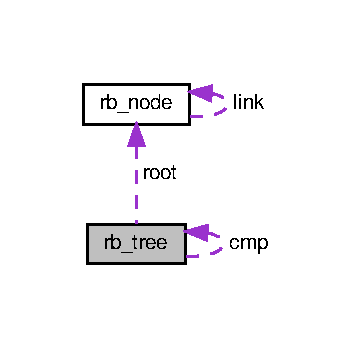
\includegraphics[width=169pt]{structrb__tree__coll__graph}
\end{center}
\end{figure}
\subsection*{Public Attributes}
\begin{DoxyCompactItemize}
\item 
\mbox{\Hypertarget{structrb__tree_aaa514d45d7d3fb00e0b01bce1e2130a0}\label{structrb__tree_aaa514d45d7d3fb00e0b01bce1e2130a0}} 
struct \hyperlink{structrb__node}{rb\+\_\+node} $\ast$ {\bfseries root}
\item 
\mbox{\Hypertarget{structrb__tree_a12b25635842ed1188e9b9598d47443e6}\label{structrb__tree_a12b25635842ed1188e9b9598d47443e6}} 
rb\+\_\+tree\+\_\+node\+\_\+cmp\+\_\+f {\bfseries cmp}
\item 
\mbox{\Hypertarget{structrb__tree_ab58b3455854ba1d62d56a9edb633fe00}\label{structrb__tree_ab58b3455854ba1d62d56a9edb633fe00}} 
size\+\_\+t {\bfseries size}
\item 
\mbox{\Hypertarget{structrb__tree_ab35a7ecb250e880e514364c254ec7a19}\label{structrb__tree_ab35a7ecb250e880e514364c254ec7a19}} 
void $\ast$ {\bfseries info}
\end{DoxyCompactItemize}


The documentation for this struct was generated from the following file\+:\begin{DoxyCompactItemize}
\item 
src/map/rb\+\_\+tree.\+h\end{DoxyCompactItemize}

\hypertarget{structimpl_1_1TestCount}{}\section{impl\+:\+:Test\+Count$<$ I, bool $>$ Struct Template Reference}
\label{structimpl_1_1TestCount}\index{impl\+::\+Test\+Count$<$ I, bool $>$@{impl\+::\+Test\+Count$<$ I, bool $>$}}


\subsection{Detailed Description}
\subsubsection*{template$<$int I, bool = test\+Exists$<$\+Test\+Suite$<$\+I$>$$>$()$>$\newline
struct impl\+::\+Test\+Count$<$ I, bool $>$}

Vérifier que le test I existe. Assume que chaque test $<$ I existe. 

The documentation for this struct was generated from the following file\+:\begin{DoxyCompactItemize}
\item 
src/test/Equivalence.\+cpp\end{DoxyCompactItemize}

\hypertarget{structimpl_1_1TestCount_3_01I_00_01false_01_4}{}\section{impl\+:\+:Test\+Count$<$ I, false $>$ Struct Template Reference}
\label{structimpl_1_1TestCount_3_01I_00_01false_01_4}\index{impl\+::\+Test\+Count$<$ I, false $>$@{impl\+::\+Test\+Count$<$ I, false $>$}}
\subsection*{Public Types}
\begin{DoxyCompactItemize}
\item 
\mbox{\Hypertarget{structimpl_1_1TestCount_3_01I_00_01false_01_4_aa02a02a012f021a76cec2a13911ca4b7}\label{structimpl_1_1TestCount_3_01I_00_01false_01_4_aa02a02a012f021a76cec2a13911ca4b7}} 
enum \{ {\bfseries count} = I
 \}
\end{DoxyCompactItemize}
\subsection*{Static Public Member Functions}
\begin{DoxyCompactItemize}
\item 
\mbox{\Hypertarget{structimpl_1_1TestCount_3_01I_00_01false_01_4_a788ccb8cc8b9f3851b36963ef04a35fc}\label{structimpl_1_1TestCount_3_01I_00_01false_01_4_a788ccb8cc8b9f3851b36963ef04a35fc}} 
static void {\bfseries do\+Next\+Test} (bool $\ast$)
\end{DoxyCompactItemize}


The documentation for this struct was generated from the following file\+:\begin{DoxyCompactItemize}
\item 
src/test/Equivalence.\+cpp\end{DoxyCompactItemize}

\hypertarget{structimpl_1_1TestCount_3_01I_00_01true_01_4}{}\section{impl\+:\+:Test\+Count$<$ I, true $>$ Struct Template Reference}
\label{structimpl_1_1TestCount_3_01I_00_01true_01_4}\index{impl\+::\+Test\+Count$<$ I, true $>$@{impl\+::\+Test\+Count$<$ I, true $>$}}
\subsection*{Public Types}
\begin{DoxyCompactItemize}
\item 
\mbox{\Hypertarget{structimpl_1_1TestCount_3_01I_00_01true_01_4_a74bc23e9df8e6408a4609f77e1ae79f8}\label{structimpl_1_1TestCount_3_01I_00_01true_01_4_a74bc23e9df8e6408a4609f77e1ae79f8}} 
enum \{ {\bfseries count} = Test\+Count$<$I + 1$>$\+:\+:count
 \}
\end{DoxyCompactItemize}
\subsection*{Static Public Member Functions}
\begin{DoxyCompactItemize}
\item 
static void \hyperlink{structimpl_1_1TestCount_3_01I_00_01true_01_4_a49739cfdb5be878f725d73b2ef4743ef}{do\+Next\+Test} (bool $\ast$resultats)
\end{DoxyCompactItemize}


\subsection{Member Function Documentation}
\mbox{\Hypertarget{structimpl_1_1TestCount_3_01I_00_01true_01_4_a49739cfdb5be878f725d73b2ef4743ef}\label{structimpl_1_1TestCount_3_01I_00_01true_01_4_a49739cfdb5be878f725d73b2ef4743ef}} 
\index{impl\+::\+Test\+Count$<$ I, true $>$@{impl\+::\+Test\+Count$<$ I, true $>$}!do\+Next\+Test@{do\+Next\+Test}}
\index{do\+Next\+Test@{do\+Next\+Test}!impl\+::\+Test\+Count$<$ I, true $>$@{impl\+::\+Test\+Count$<$ I, true $>$}}
\subsubsection{\texorpdfstring{do\+Next\+Test()}{doNextTest()}}
{\footnotesize\ttfamily template$<$int I$>$ \\
static void \hyperlink{structimpl_1_1TestCount}{impl\+::\+Test\+Count}$<$ I, true $>$\+::do\+Next\+Test (\begin{DoxyParamCaption}\item[{bool $\ast$}]{resultats }\end{DoxyParamCaption})\hspace{0.3cm}{\ttfamily [inline]}, {\ttfamily [static]}}

Effectue le test n°\{I\}, puis le test suivant s\textquotesingle{}il existe.


\begin{DoxyParams}[1]{Parameters}
\mbox{\tt out}  & {\em resultats} & L\textquotesingle{}ensemble des résultats des tests affecte à resultats\mbox{[}I\mbox{]} le résultat du test n°\{I\}\\
\hline
\end{DoxyParams}

\begin{DoxyTemplParams}{Template Parameters}
{\em I} & le test à vérifier \\
\hline
\end{DoxyTemplParams}


The documentation for this struct was generated from the following file\+:\begin{DoxyCompactItemize}
\item 
src/test/Equivalence.\+cpp\end{DoxyCompactItemize}

\hypertarget{structTestSuite}{}\section{Test\+Suite$<$ N $>$ Struct Template Reference}
\label{structTestSuite}\index{Test\+Suite$<$ N $>$@{Test\+Suite$<$ N $>$}}
\subsection*{Public Types}
\begin{DoxyCompactItemize}
\item 
\mbox{\Hypertarget{structTestSuite_a0bc1f544eed95074c61943848b66ba11}\label{structTestSuite_a0bc1f544eed95074c61943848b66ba11}} 
enum \{ {\bfseries empty\+Test} = 1
 \}
\end{DoxyCompactItemize}
\subsection*{Public Member Functions}
\begin{DoxyCompactItemize}
\item 
{\footnotesize template$<$typename multimap\+\_\+t $>$ }\\multimap\+\_\+t \hyperlink{structTestSuite_a791fd382a8eb4d1f4f8d75369d3125dd}{operator()} ()=delete
\end{DoxyCompactItemize}


\subsection{Detailed Description}
\subsubsection*{template$<$int N$>$\newline
struct Test\+Suite$<$ N $>$}

Foncteur qui permet d\textquotesingle{}effectuer une suite d\textquotesingle{}opération sur une multimap. 
\begin{DoxyTemplParams}{Template Parameters}
{\em N} & Indice de la suite d\textquotesingle{}opération à tester. L\textquotesingle{}ensemble des suites d\textquotesingle{}opérations \hyperlink{structTestSuite}{Test\+Suite}{\itshape  ou I appartient à \mbox{[}0;n\mbox{]} sera testé (consécutive) Où \{n\} est un entier positif, Et où chaque classe \hyperlink{structTestSuite}{Test\+Suite}{\itshape  est spécialisée et comporte un operator(). }}\\
\hline
\end{DoxyTemplParams}


\subsection{Member Function Documentation}
\mbox{\Hypertarget{structTestSuite_a791fd382a8eb4d1f4f8d75369d3125dd}\label{structTestSuite_a791fd382a8eb4d1f4f8d75369d3125dd}} 
\index{Test\+Suite@{Test\+Suite}!operator()@{operator()}}
\index{operator()@{operator()}!Test\+Suite@{Test\+Suite}}
\subsubsection{\texorpdfstring{operator()()}{operator()()}}
{\footnotesize\ttfamily template$<$int N$>$ \\
template$<$typename multimap\+\_\+t $>$ \\
multimap\+\_\+t \hyperlink{structTestSuite}{Test\+Suite}$<$ N $>$\+::operator() (\begin{DoxyParamCaption}{ }\end{DoxyParamCaption})\hspace{0.3cm}{\ttfamily [delete]}}

Générer la multimap de test. Pour la structure générique, on considère que le test n\textquotesingle{}existe pas, Il faut surcharger la classe pour en définir un ce qui est détecté par S\+F\+I\+N\+AE si le membre empty\+Test existe.


\begin{DoxyTemplParams}{Template Parameters}
{\em multimap\+\_\+t} & un type générique de \hyperlink{classMultimap}{Multimap} \\
\hline
\end{DoxyTemplParams}
\begin{DoxyReturn}{Returns}
La multimap généré à l\textquotesingle{}issu de l\textquotesingle{}algorithme. 
\end{DoxyReturn}


The documentation for this struct was generated from the following file\+:\begin{DoxyCompactItemize}
\item 
src/test/Equivalence.\+cpp\end{DoxyCompactItemize}

\hypertarget{structTestSuite_3_010_01_4}{}\section{Test\+Suite$<$ 0 $>$ Struct Template Reference}
\label{structTestSuite_3_010_01_4}\index{Test\+Suite$<$ 0 $>$@{Test\+Suite$<$ 0 $>$}}
\subsection*{Public Member Functions}
\begin{DoxyCompactItemize}
\item 
\mbox{\Hypertarget{structTestSuite_3_010_01_4_a857db883aaf9f7f4248f0fb280b34798}\label{structTestSuite_3_010_01_4_a857db883aaf9f7f4248f0fb280b34798}} 
{\footnotesize template$<$typename multimap\+\_\+t $>$ }\\multimap\+\_\+t {\bfseries operator()} ()
\end{DoxyCompactItemize}


\subsection{Detailed Description}
\subsubsection*{template$<$$>$\newline
struct Test\+Suite$<$ 0 $>$}

Premier test, tester sur les insertions et suppressions d\textquotesingle{}intervalles 

The documentation for this struct was generated from the following file\+:\begin{DoxyCompactItemize}
\item 
src/test/Equivalence.\+cpp\end{DoxyCompactItemize}

\hypertarget{structTestSuite_3_011_01_4}{}\section{Test\+Suite$<$ 1 $>$ Struct Template Reference}
\label{structTestSuite_3_011_01_4}\index{Test\+Suite$<$ 1 $>$@{Test\+Suite$<$ 1 $>$}}
\subsection*{Public Member Functions}
\begin{DoxyCompactItemize}
\item 
\mbox{\Hypertarget{structTestSuite_3_011_01_4_aa195cba888d14e59594dbc164f7de927}\label{structTestSuite_3_011_01_4_aa195cba888d14e59594dbc164f7de927}} 
{\footnotesize template$<$typename multimap\+\_\+t $>$ }\\multimap\+\_\+t {\bfseries operator()} ()
\end{DoxyCompactItemize}


\subsection{Detailed Description}
\subsubsection*{template$<$$>$\newline
struct Test\+Suite$<$ 1 $>$}

Deuxième test, insertions et suppressions aléatoires manuelles 

The documentation for this struct was generated from the following file\+:\begin{DoxyCompactItemize}
\item 
src/test/Equivalence.\+cpp\end{DoxyCompactItemize}

\hypertarget{classMultimap_1_1value__compare}{}\section{Multimap$<$ Key, T, Compare $>$\+:\+:value\+\_\+compare Class Reference}
\label{classMultimap_1_1value__compare}\index{Multimap$<$ Key, T, Compare $>$\+::value\+\_\+compare@{Multimap$<$ Key, T, Compare $>$\+::value\+\_\+compare}}


Classe qui compare les paires.  




{\ttfamily \#include $<$Multimap.\+h$>$}

\subsection*{Public Types}
\begin{DoxyCompactItemize}
\item 
\mbox{\Hypertarget{classMultimap_1_1value__compare_a8a34051443c474d05e7864feed1b6d81}\label{classMultimap_1_1value__compare_a8a34051443c474d05e7864feed1b6d81}} 
typedef bool {\bfseries result\+\_\+type}
\item 
\mbox{\Hypertarget{classMultimap_1_1value__compare_a194d5ffd210c7ab77b3119cedb22c51a}\label{classMultimap_1_1value__compare_a194d5ffd210c7ab77b3119cedb22c51a}} 
typedef value\+\_\+type {\bfseries first\+\_\+argument\+\_\+type}
\item 
\mbox{\Hypertarget{classMultimap_1_1value__compare_af2ba2cc0bed81b3772371bfb13350dbe}\label{classMultimap_1_1value__compare_af2ba2cc0bed81b3772371bfb13350dbe}} 
typedef value\+\_\+type {\bfseries second\+\_\+argument\+\_\+type}
\end{DoxyCompactItemize}
\subsection*{Public Member Functions}
\begin{DoxyCompactItemize}
\item 
\mbox{\Hypertarget{classMultimap_1_1value__compare_a86e3025154d686741ad33e78f80d1c13}\label{classMultimap_1_1value__compare_a86e3025154d686741ad33e78f80d1c13}} 
bool {\bfseries operator()} (const value\+\_\+type \&lhs, const value\+\_\+type \&rhs) const
\end{DoxyCompactItemize}
\subsection*{Protected Member Functions}
\begin{DoxyCompactItemize}
\item 
\mbox{\Hypertarget{classMultimap_1_1value__compare_a48661dffd6e198a2dd96ff172f0d5d44}\label{classMultimap_1_1value__compare_a48661dffd6e198a2dd96ff172f0d5d44}} 
{\bfseries value\+\_\+compare} (Compare c)
\end{DoxyCompactItemize}
\subsection*{Protected Attributes}
\begin{DoxyCompactItemize}
\item 
\mbox{\Hypertarget{classMultimap_1_1value__compare_a29c103107b387e1f8620f573f47f9591}\label{classMultimap_1_1value__compare_a29c103107b387e1f8620f573f47f9591}} 
Compare {\bfseries comp}
\end{DoxyCompactItemize}
\subsection*{Friends}
\begin{DoxyCompactItemize}
\item 
\mbox{\Hypertarget{classMultimap_1_1value__compare_a922410cc20fad40c7a00e23639f4e5ac}\label{classMultimap_1_1value__compare_a922410cc20fad40c7a00e23639f4e5ac}} 
class {\bfseries Multimap}
\end{DoxyCompactItemize}


\subsection{Detailed Description}
\subsubsection*{template$<$class Key, class T, class Compare$>$\newline
class Multimap$<$ Key, T, Compare $>$\+::value\+\_\+compare}

Classe qui compare les paires. 

The documentation for this class was generated from the following file\+:\begin{DoxyCompactItemize}
\item 
src/multimap/Multimap.\+h\end{DoxyCompactItemize}

%--- End generated contents ---

% Index
\backmatter
\newpage
\phantomsection
\clearemptydoublepage
\addcontentsline{toc}{chapter}{Index}
\printindex

\end{document}
